\documentclass[11pt,a4paper]{article}

% ------------------------------------------------------------------ packages
\usepackage[T1]{fontenc}
\usepackage[utf8]{inputenc}
\usepackage{lmodern}
\usepackage{microtype}
\usepackage[htt]{hyphenat}
\usepackage[margin=2.4cm]{geometry}
\usepackage{amsmath,amssymb}
\usepackage{booktabs,longtable,tabularx,array,multirow}
\usepackage{graphicx}
\usepackage[section]{placeins}
\usepackage{xcolor}
\usepackage{enumitem}
\usepackage{tikz}
\usetikzlibrary{arrows.meta,positioning,fit,calc,shapes.geometric,backgrounds}
\usepackage{listings}
\usepackage[most]{tcolorbox}
\usepackage{csquotes}
\usepackage[backend=biber,style=ieee,maxnames=4]{biblatex}
\addbibresource{references.bib}
\usepackage{fancyhdr}
\usepackage{titlesec}
\usepackage[hidelinks]{hyperref}
\usepackage[nameinlink,capitalise]{cleveref}

\definecolor{ink}{HTML}{1F2A44}
\definecolor{accent}{HTML}{B5532A}
\definecolor{soft}{HTML}{EEF1F6}
\definecolor{okgreen}{HTML}{2E7D4F}

\titleformat{\section}{\Large\bfseries\color{ink}}{\thesection}{0.8em}{}
\titleformat{\subsection}{\large\bfseries\color{ink}}{\thesubsection}{0.7em}{}
\setlength{\parskip}{0.45em}
\setlength{\parindent}{0pt}
\setlist{itemsep=0.15em,topsep=0.3em}
\renewcommand{\arraystretch}{1.15}

\pagestyle{fancy}
\fancyhf{}
\fancyhead[L]{\small\color{ink}CustodyChain: Evidence Fingerprinting}
\fancyhead[R]{\small\color{ink}Internal discussion draft}
\fancyfoot[C]{\small\thepage}

\lstdefinestyle{json}{basicstyle=\ttfamily\scriptsize,breaklines=true,columns=fullflexible,
  frame=single,rulecolor=\color{gray!40},backgroundcolor=\color{soft},showstringspaces=false}

\newtcolorbox{keypoint}[1][]{colback=soft,colframe=ink,boxrule=0.6pt,arc=2pt,left=6pt,right=6pt,top=4pt,bottom=4pt,fonttitle=\bfseries,title=#1}
\newtcolorbox{caution}[1][]{colback=accent!6,colframe=accent,boxrule=0.6pt,arc=2pt,left=6pt,right=6pt,top=4pt,bottom=4pt,fonttitle=\bfseries,title=#1}

\newcommand{\Hash}{\mathsf{H}}
\newcommand{\shatwo}{\textsc{sha-256}}
\newcommand{\shathree}{\textsc{sha3-256}}
\newcommand{\code}[1]{\texttt{#1}}

\newcommand{\NbManifestHash}{d5b719250e11dda255782f9fa1d4b77d746ae94d7a5bc5232df470b2e902ade1}
\newcommand{\NbMerkleRoot}{6e8451494a032e3317bc66df35c259c968a35e2fc67832d4f079695e9c514102}
\newcommand{\PhotoManifestHash}{97d115c039aae8de9b250e6e80ff7ee9cc2aeb203842891aa24f42c20be51cd2}
\newcommand{\PhotoSha}{0ee550034602fa2da9f6716c4cead703e14cb47b3dcead1cbfda0eb1bf68b605}
\newcommand{\PhotoPhash}{e94a86b1b1ce39b1}
\newcommand{\KnifeRefPoints}{16000}
\newcommand{\KnifeRuleRms}{0.60}
\newcommand{\KnifeRuleMax}{3.00}
\newcommand{\NbRescanMaxDist}{4}
\newcommand{\NbForgedDist}{20}
\newcommand{\PhotoSecondDist}{0}
\newcommand{\PhotoTamperDist}{0}
\newcommand{\PhotoOtherDist}{28}
\newcommand{\PhotoResaveDist}{0}


\title{\color{ink}\textbf{Fingerprinting Real-World Evidence for a\\Permissioned Chain-of-Custody Ledger}\\[0.4em]
\large How hashes are computed for physical and digital evidence, what they prove,\\ the input specification, and how the CustodyChain network will run}
\author{CustodyChain project\\\small Internal discussion document (draft v0.1)}
\date{19 November 2026}

\begin{document}
\maketitle
\thispagestyle{empty}

\begin{abstract}
\noindent A blockchain does not hold evidence. It holds \emph{fingerprints} of evidence and a record of who did what to it, and when. This document sets out precisely how those fingerprints are produced for each class of evidence we expect to handle: crime-scene photographs, search-and-seizure video, CCTV exports, recovered documents such as notebooks, general physical items, biological samples, seized devices, forensic images, mobile extractions, cloud data, IoT logs and procedural paperwork. We separate two questions that are often confused. The first is whether a record has been altered (\emph{integrity}), which exact cryptographic hashes answer. The second is whether this is the same physical item (\emph{identity}), which hashes cannot answer and which needs tolerant comparison of new captures against reference captures. This separation is what resolves the objection that \enquote{no two photographs are ever the same}. We define a canonical, schema-validated \emph{evidence manifest} for each item. Its \shatwo{} digest and a salted Merkle root over its files are the only evidence data anchored on the ledger. We map the design to the Bharatiya Nagarik Suraksha Sanhita and Bharatiya Sakshya Adhiniyam (including the Section 63 certificate), state the residual risks, and describe the planned Byzantine-fault-tolerant network of four consensus nodes operated by separate agencies. Every number in the worked examples was computed by the reference tool that accompanies this document.
\end{abstract}

\tableofcontents
\newpage

\section{Introduction}
\label{sec:intro}

\subsection{Purpose of this document}
CustodyChain began as a reproduction of the Hyperledger Fabric chain-of-custody prototype of Loffi et al.~\cite{loffi2025}. Reproducing it showed that the prototype stores free-text \enquote{5W1H} records and nothing that ties a record to the evidence it describes. There is no hash of a file, no description of how a physical object is identified, and no rule about which inputs are mandatory. That gap is the subject of this document. Before more smart-contract code is written we need clarity on four questions:

\begin{enumerate}[label=\textbf{Q\arabic*}]
  \item \textbf{What exactly is hashed} for each kind of evidence, given that the ledger can only ever hold a fingerprint of the evidence and never the evidence itself?
  \item \textbf{What a hash does and does not prove}, and in particular how physical evidence is handled when \enquote{no two photographs are ever the same}.
  \item \textbf{Which inputs are mandatory} at each stage and for each evidence type, so that the system has a well-defined input contract rather than free text.
  \item \textbf{How the network runs}: which consensus algorithm, how many nodes, run by whom, and how the ledger persists.
\end{enumerate}

This is an internal discussion draft. It aims to be precise enough to implement from, and explicit about what is a design decision, what is a recommendation and what is still open (\cref{sec:limits}).

\subsection{Decisions already taken}
The following decisions were agreed after the project meeting of November 2026 and are assumed throughout.

\begin{center}
\begin{tabularx}{\linewidth}{@{}lX@{}}
\toprule
Topic & Decision \\
\midrule
Consensus & Byzantine fault tolerant (BFT) ordering with \textbf{four consensus nodes}, the minimum for tolerating one faulty node ($n = 3f+1$, $f=1$). Implemented and tested (\cref{sec:netstatus}). \\
Organisations & Real agencies are modelled (test phase): Police, Forensic Science Laboratory (FSL), Court and Prosecution each operate one consensus node. \\
Hardware & A single laptop for the test phase. \\
Persistence & Ledger and identities must survive restarts of Docker or the host. Wiping is a separate, explicit operation. This is implemented and tested (\cref{sec:persistence}). \\
Fingerprints & Both \emph{integrity} hashes and \emph{identity} fingerprints are required (\cref{sec:twolayer}). \\
Legal frame & The Indian criminal-procedure and evidence framework (BNSS, BSA) is in scope (\cref{sec:legal}). \\
\bottomrule
\end{tabularx}
\end{center}

\subsection{Summary of the proposal}
\begin{keypoint}[The design in five sentences]
\begin{enumerate}[nosep,leftmargin=*]
  \item Every evidence item is documented by a set of \emph{artefacts}: files such as photographs, scans, 3D scans, videos, forensic images and documents. Each artefact is hashed with \shatwo{} and \shathree{} at the earliest possible moment, ideally on the capture device.
  \item The artefacts, the case and collection facts, and class-specific attributes are written into a schema-validated \emph{evidence manifest}. The manifest is serialised canonically (RFC~8785) and hashed, and its artefacts are bound by a salted Merkle tree (RFC~6962).
  \item Only the manifest hash and the Merkle root, plus the custody events that follow, go on the ledger. Files and manifests stay off-chain in encrypted evidence storage.
  \item Exact hashes prove that \emph{records} have not been altered. Whether a \emph{physical item} is the same one that was seized is established separately, by comparing new captures with the reference captures (perceptual image hashes, 3D-scan deviation, seal and label identifiers) under declared, calibrated thresholds. The result is recorded as a custody event.
  \item The ledger is ordered by a BFT consensus of four agency-operated nodes, so no single agency can rewrite, reorder or suppress the history.
\end{enumerate}
\end{keypoint}

\subsection{Status of this draft}
Version 0.2 adds the implementation of the prototype (\cref{sec:impl}) and its evaluation (\cref{sec:eval}). The prototype implements the two-layer model, the input specification, the custody lifecycle with two-agency transfers, identity checks and court outputs on the four-agency BFT network; how to run it is described in \code{CustodyChain/PROTOTYPE.md}.

\subsection{Accompanying artefacts}
This report is accompanied by a machine-readable input specification, a reference tool and worked examples. All of these live in the project repository under \code{outputs/}.
\begin{itemize}
  \item \code{spec/evidence-manifest.schema.json} and \code{spec/custody-event.schema.json}: JSON Schema (draft 2020-12) definitions of the inputs. \Cref{app:spec} is generated from them.
  \item \code{tools/evidence\_hash.py}: the reference implementation of hashing, canonicalisation, Merkle trees and proofs, verification, perceptual hashing and 3D-scan comparison.
  \item \code{tools/make\_worked\_examples.py}: generates the synthetic evidence and every number in \cref{sec:worked}.
\end{itemize}

\section{The problem: what must be protected, against whom}
\label{sec:problem}

\subsection{The evidence lifecycle}
Evidence passes through identification and collection, packaging and sealing, transport, storage, forensic examination (which may create \emph{derived} evidence such as a forensic image or an aliquot of a sample), presentation in court, and finally return, archival or disposal. At every transition there must be a record of what the item was, who held it, what was done to it and why, so that the item produced in court can be shown to be the item that was collected, in a known condition~\cite{iso27037,sopbnss}. \Cref{tab:stages} restates the project brief's stage analysis and adds the control this design contributes at each stage.

\begin{table}[htbp]
\centering\small
\begin{tabularx}{\linewidth}{@{}l>{\raggedright}p{2.6cm}>{\raggedright}p{2.5cm}>{\raggedright}p{2.6cm}X@{}}
\toprule
Stage & What must be protected & Threat & Existing mechanism & Contribution of this design \\
\midrule
Collection & Original evidence and its metadata & Fabrication, alteration, omission & Seizure memo, witnesses, A/V recording (BNSS s.105) & Hash at capture; manifest binds captures, seals, witnesses and the A/V recording; anchored within minutes \\
Storage & Evidence and its record & Tampering, deletion, substitution & Malkhana registers, secure storage & Off-chain store verified against ledger hashes; append-only events \\
Transfer & Custody record & Unauthorised handling, gaps & Paper chain-of-custody form & Two-phase transfer (initiate and accept) signed by both custodians' certificates; seal state recorded \\
Examination & Original and derived evidence & Modification, undocumented processing & Hashing, lab notes & Derived items get their own manifests linked to the parent; verify-identity events on receipt \\
Court & Authenticity & Disputes over provenance & BSA s.63 certificate & Certificate fields are generated from the manifest; independent re-verification against the ledger \\
Archival & Long-term integrity & Loss, bit-rot, algorithm ageing & Archival systems & Dual hashes (\shatwo{} and \shathree{}); periodic re-verification events; algorithm agility \\
\bottomrule
\end{tabularx}
\caption{Lifecycle stages, threats and controls (extends the project brief).}
\label{tab:stages}
\end{table}

\subsection{Adversaries}
The design must hold against the following parties.
\begin{description}[style=nextline,leftmargin=1.2em]
  \item[A1: Dishonest custodian (insider).] A person with legitimate access who substitutes an item, edits a file, back-dates a record or quietly removes a page. This is the most realistic threat.
  \item[A2: Dishonest agency administrator.] Someone controlling one organisation's infrastructure, including its ledger node, who tries to rewrite, reorder or censor history.
  \item[A3: External attacker.] Compromises a server or storage system.
  \item[A4: Opposing party in court.] Not malicious toward the system, but motivated to challenge provenance. The system must give a judge something \emph{independently verifiable} rather than \enquote{trust our database}.
\end{description}

\subsection{What a hash proves, and what it does not}
\label{sec:whathashproves}
A cryptographic hash of a file proves exactly one thing: the file presented now is bit-for-bit identical to the file that was hashed earlier. As Burri et al.\ put it, the hash value alone \enquote{does not prove that digital evidence is the same as when it was obtained, only that the contents has not been modified since the time when the hash was calculated}~\cite{burri2020}. Three consequences follow, and the rest of the design is built around them.
\begin{enumerate}
  \item \textbf{The time of hashing matters.} Anything done to a file before it is hashed is invisible. The interval between capture and the first hash, and between the first hash and anchoring on the ledger, is a window of vulnerability that must be minimised and recorded (\cref{sec:window}).
  \item \textbf{A hash says nothing about truthfulness.} A staged photograph hashed at capture is a perfectly intact staged photograph. Blockchains preserve whatever is entered at collection; the controls at collection (witnesses, continuous A/V recording, device-generated hashes) carry that burden (\cref{sec:limits}).
  \item \textbf{A physical object cannot be hashed.} Only digital captures \emph{of} it can. Whether an object in court is the object that was seized is a different question with a different (probabilistic) answer (\cref{sec:twolayer}).
\end{enumerate}

\subsection{Requirements}
\label{sec:requirements}
\begin{center}\small
\begin{tabularx}{\linewidth}{@{}lX@{}}
\toprule
ID & Requirement \\
\midrule
R1 & Every artefact is fingerprinted with an exact, collision-resistant hash at the earliest practicable point, with the time and place of hashing recorded. \\
R2 & Every evidence item has one canonical, machine-validated record (the manifest) whose fingerprint is anchored on the ledger. \\
R3 & Physical items have a declared re-identification method with an explicit acceptance rule, and every re-identification is itself recorded. \\
R4 & The actor and time of every custody event come from the transaction (certificate and transaction timestamp), never from user input. \\
R5 & History is append-only: corrections are new events; nothing is updated or deleted on the ledger. \\
R6 & No single agency can rewrite, reorder or suppress ledger history. \\
R7 & The ledger holds no evidence content and no low-entropy personal data in clear; disclosure is need-to-know. \\
R8 & A third party (court, defence expert) can verify any artefact against the ledger with standard tools and without trusting the operator. \\
R9 & The outputs required by BNSS/BSA procedure, notably the s.63(4)(c) certificate fields, can be produced directly from the records. \\
R10 & Hash algorithms can be replaced without invalidating existing records (algorithm agility). \\
\bottomrule
\end{tabularx}
\end{center}

\section{Cryptographic background}
\label{sec:background}

\subsection{Hash functions and their security properties}
A cryptographic hash function $\Hash : \{0,1\}^* \to \{0,1\}^n$ maps an input of any length to a fixed-length digest (here $n = 256$). For evidence work three properties matter:
\begin{description}[style=nextline,leftmargin=1.2em]
  \item[Pre-image resistance.] Given $h$, it is infeasible to find any $x$ with $\Hash(x) = h$ (about $2^{n}$ work).
  \item[Second pre-image resistance.] Given $x$, it is infeasible to find $x' \neq x$ with $\Hash(x') = \Hash(x)$ (about $2^{n}$ work). This is the property that stops a custodian from substituting a different file with the same hash.
  \item[Collision resistance.] It is infeasible to find any pair $x \neq x'$ with $\Hash(x) = \Hash(x')$ (about $2^{n/2}$ work by the birthday bound). This matters when the adversary can influence the original. For example, a person preparing two versions of a document in advance could have one hashed and later produce the other.
\end{description}
The \emph{avalanche} behaviour of a good hash, where changing one input bit flips about half of the output bits, is why a single altered pixel, EXIF field or sector produces a completely unrelated digest (\cref{sec:worked}).

\paragraph{Algorithm choice.} \shatwo{} (SHA-2 family, FIPS~180-4~\cite{fips180}) offers 128-bit collision resistance and is the algorithm named explicitly in the BSA Schedule certificate~\cite{bsa2023}. \textsc{md5} and \textsc{sha-1}, which the same certificate also lists, are \textbf{broken for collision resistance}. Practical \textsc{md5} collisions have been known since 2004--05~\cite{wang2005}, and a full \textsc{sha-1} collision was published in 2017~\cite{stevens2017}. They may still appear in tool reports for cross-reference, but they must never be the sole fingerprint. We record \emph{two} independent digests per artefact: \shatwo{} and \shathree{} (Keccak, FIPS~202~\cite{fips202}). The two have unrelated internal designs, so a future weakness in one does not immediately compromise records, which addresses R10.

\subsection{Canonical serialisation}
Hashing structured data (a manifest) requires that the same logical content always produces the same bytes. JSON permits arbitrary key order, whitespace and number formats, so we use the JSON Canonicalization Scheme (JCS, RFC~8785~\cite{rfc8785}). JCS sorts keys by UTF-16 code units, uses no insignificant whitespace, and fixes string escaping and number serialisation. To remove floating-point ambiguity entirely, our manifests forbid floating-point numbers: decimals such as \code{"148.5"} grams are carried as strings. The \emph{manifest hash} is $\shatwo(\mathrm{JCS}(M))$.

\subsection{Merkle trees}
A Merkle tree~\cite{merkle1987} hashes a list of leaves pairwise up to a single \emph{root}. Changing any leaf changes the root. Any single leaf can be proven to belong to the root by revealing only $\lceil \log_2 N \rceil$ sibling hashes (an \emph{inclusion proof}), without revealing the other leaves. We use the exact construction of Certificate Transparency (RFC~6962~\cite{rfc6962}, verified per RFC~9162~\cite{rfc9162}):
\begin{align*}
\mathrm{MTH}(\{d_0\}) &= \shatwo(\texttt{0x00} \,\|\, d_0), \\
\mathrm{MTH}(D_{[0:n]}) &= \shatwo\big(\texttt{0x01} \,\|\, \mathrm{MTH}(D_{[0:k]}) \,\|\, \mathrm{MTH}(D_{[k:n]})\big), \quad k = \text{largest power of 2} < n.
\end{align*}
The \texttt{0x00}/\texttt{0x01} prefixes provide domain separation, so a leaf can never be passed off as an internal node (second-pre-image attacks on naive Merkle trees). Our leaves are \emph{salted}:
\[
d_i = s_i \,\|\, \mathrm{id}_i \,\|\, \shatwo(\text{artefact}_i), \qquad s_i \xleftarrow{\$} \{0,1\}^{256}.
\]
The salt $s_i$ is kept off-chain in the manifest. It prevents someone who holds a candidate file (for example a known image) from confirming, using only ledger data, that the file is part of a case. This is the same privacy idea as the salted hashes of Burri et al.~\cite{burri2020}.

For very large single files (video, disk images) the same tree can be built over fixed-size chunks (\emph{chunk Merkle root}), so damage can be localised to a chunk rather than merely detected (\cref{sec:worked}).

\subsection{Signatures, identity and time}
Hyperledger Fabric is permissioned. Every participant holds an X.509 certificate issued by its organisation's certificate authority, and organisations are represented on the channel by Membership Service Providers (MSPs)~\cite{androulaki2018}. Every transaction is signed by the submitting client and by the endorsing peers. The chaincode can therefore take the \emph{actor} of an event from the signer's certificate (\code{ctx.clientIdentity}) and the \emph{time} from the transaction header (\code{ctx.stub.getTxTimestamp()}), which satisfies R4. The transaction timestamp is set by the client and checked by the network, and is not a trusted timestamp in the RFC~3161 sense~\cite{rfc3161}. Its integrity comes from the block order agreed by consensus. Where an independent trusted time is needed (for example, to prove a hash existed before a specific instant to a party outside the network), the manifest hash can additionally be time-stamped by an RFC~3161 Time-Stamping Authority.

\subsection{Perceptual fingerprints and geometric comparison}
\label{sec:perceptual}
A \emph{perceptual hash} maps similar-looking images to similar short codes. We use the DCT-based 64-bit pHash~\cite{zauner2010}. The image is reduced to $32\times32$ grey levels and a 2-D discrete cosine transform is taken. The $8\times8$ lowest-frequency coefficients are kept, and each bit records whether a coefficient exceeds the median of the 63 AC coefficients. Similarity is the Hamming distance $d_H \in [0,64]$. Re-photographing or re-scanning the same object yields small $d_H$; different content yields large $d_H$.

For 3D scans we rigidly align the new scan to the reference with the Iterative Closest Point (ICP) algorithm~\cite{besl1992}, initialised from principal axes. We then measure the \emph{symmetric} nearest-neighbour deviation, reporting RMS, 95th percentile and maximum. The comparison must be symmetric. Distances from the new scan to the reference reveal added or displaced material. Only distances from the reference to the new scan reveal \emph{missing} material such as a nick or a broken tip; our first implementation measured one direction only and accepted a damaged knife as a match, an error the worked example now guards against.

\begin{caution}[Perceptual and geometric fingerprints are not integrity proofs]
They are designed to \emph{tolerate} change. An image from which an object has been digitally removed can have the same perceptual hash as the original (\cref{tab:photo}: Hamming distance \PhotoTamperDist{}). They serve only to re-identify; integrity is always established by exact hashes.
\end{caution}

\section{The two-layer fingerprinting model}
\label{sec:twolayer}

\subsection{Terms}
\begin{description}[style=nextline,leftmargin=1.2em]
  \item[Evidence item.] The thing seized or produced: a knife, a notebook, a phone, a CCTV export, a blood swab, a seizure memo. It has a globally unique \code{evidence\_id} of the form \code{GJ-GNR-CYBPS-2026-000123-E004} (state, district, unit, year, case sequence, item sequence).
  \item[Artefact.] A file that documents or constitutes the item: a photograph, a page scan, a 3D scan, a video segment, a forensic image, a provider's data package, a PDF. Artefacts are what we hash.
  \item[Manifest.] The canonical, schema-validated JSON record of one item. It contains the case and collection facts, packaging and seals, class-specific attributes, every artefact with its hashes and capture details, and the identity-fingerprint references (\cref{app:spec}).
  \item[Ledger record.] What is written on-chain: \code{evidence\_id}, class, \code{manifest\_sha256}, \code{merkle\_root}, artefact count, and the spec version. This is followed by append-only custody events.
\end{description}

\subsection{Layer 1: integrity (exact)}
For every artefact $a$ we compute $\shatwo(a)$ and $\shathree(a)$ over the exact bytes produced by the capture device, before the file is opened in any editor, renamed by software that rewrites it, or transcoded. Verification is exact:
\[
\mathrm{Verify}_{L1}(a, h) \;=\; \big[\,\shatwo(a) = h\,\big].
\]
L1 answers \emph{has this record changed since it was fingerprinted?} It has no false matches, short of breaking \shatwo{}, and no tolerance: one flipped bit is a mismatch. L1 applies to every artefact of every class, including born-digital evidence (CCTV, extractions, cloud data). For born-digital evidence the artefact \emph{is} the evidence.

\subsection{Layer 2: identity (tolerant)}
Physical objects, and the visual content of images, cannot be compared byte for byte, because every new capture differs in pose, light, noise and sampling. That is the observation that \enquote{no two photographs are ever the same}. It is correct, and it is \emph{not a problem}, because we never need to reproduce a reference capture:

\begin{keypoint}[Resolving \enquote{no two photographs are the same}]
The reference photographs, scans and 3D scans taken at seizure are themselves artefacts. They are frozen by Layer~1 at the moment of capture, and that frozen record is what is compared against later. When the item is later re-examined (on receipt at the FSL, before court), \emph{new} captures are taken. These new captures are \emph{also} frozen by Layer~1, and they are compared with the frozen references by a declared tolerant method. The comparison method, its version, the score, the threshold and the L1 hashes of the new captures are recorded in a \code{VERIFY\_IDENTITY} event. The comparison itself is therefore auditable and repeatable by anyone, including a defence expert.
\end{keypoint}

Formally, for a fingerprint extractor $\varphi$, distance $d$ and threshold $\tau$ declared in the manifest:
\[
\mathrm{Verify}_{L2}(Q, R) \;=\; \big[\, d(\varphi(Q), \varphi(R)) \le \tau \,\big],
\]
where $R$ are the reference artefacts and $Q$ the new (query) artefacts. Unlike L1, L2 has two error rates. The \emph{false match rate} (FMR) is the rate at which a different or altered item is accepted. The \emph{false non-match rate} (FNMR) is the rate at which the same item is rejected. $\tau$ trades one against the other and must be calibrated on realistic data for each method and evidence type. The thresholds used in this document are illustrative only (\cref{sec:limits}). An L2 result is \emph{evidence of identity} to be weighed by an examiner, never proof.

L2 methods by evidence type:
\begin{center}\small
\begin{tabularx}{\linewidth}{@{}lXl@{}}
\toprule
Method & Use & Rule (illustrative) \\
\midrule
\code{seal-id-exact}, \code{label-id-exact} & Tamper-evident seal numbers, barcodes and QR or RFID labels: an exact identifier physically bound to the package. The strongest and cheapest identity check, as long as the seal is intact. & exact \\
\code{serial-exact} & Manufacturer serials, IMEI, chassis numbers & exact \\
\code{phash-dct-64} & Page scans, photographs of flat items, frames & $d_H \le 10$ \\
\code{mesh-icp-rms} & 3D scans of objects (weapons, tools, footwear) & RMS $\le$ \KnifeRuleRms{} mm, max $\le$ \KnifeRuleMax{} mm \\
\code{measurement-tolerance} & Mass, dimensions & stated instrument tolerance \\
\code{keypoint-set} & Distinctive surface features matched by local descriptors (scratches, tool marks); future work & method-specific \\
\bottomrule
\end{tabularx}
\end{center}

\subsection{Binding the physical item to its digital record}
L1 and L2 operate on files; the remaining link is between the physical package and the record. Three mechanisms provide it:
\begin{enumerate}
  \item a \textbf{tamper-evident container} whose unique seal number is recorded in the manifest and re-read, with a photograph, at every transfer (\code{seal\_ids\_observed}, \code{seal\_intact});
  \item a \textbf{printed label} (QR code, optionally RFID) carrying the \code{evidence\_id}, so that scanning the package retrieves the ledger record and manifest;
  \item \textbf{continuous A/V recording of the seizure} (BNSS s.105~\cite{bnss2023}). The recording is itself an evidence item (\code{AV\_RECORDING}) referenced from each seized item's manifest, and it shows the item being packed and sealed.
\end{enumerate}

\subsection{The manifest and what goes on-chain}
\Cref{fig:flow} shows the data flow. The manifest is built from the captures and validated against the schema. Its Merkle root is computed over the salted artefact leaves and stored inside it, and the manifest is then canonicalised and hashed. The resulting pair \code{(manifest\_sha256, merkle\_root)} is submitted in the \code{REGISTER} event.

\begin{figure}[htbp]
\centering
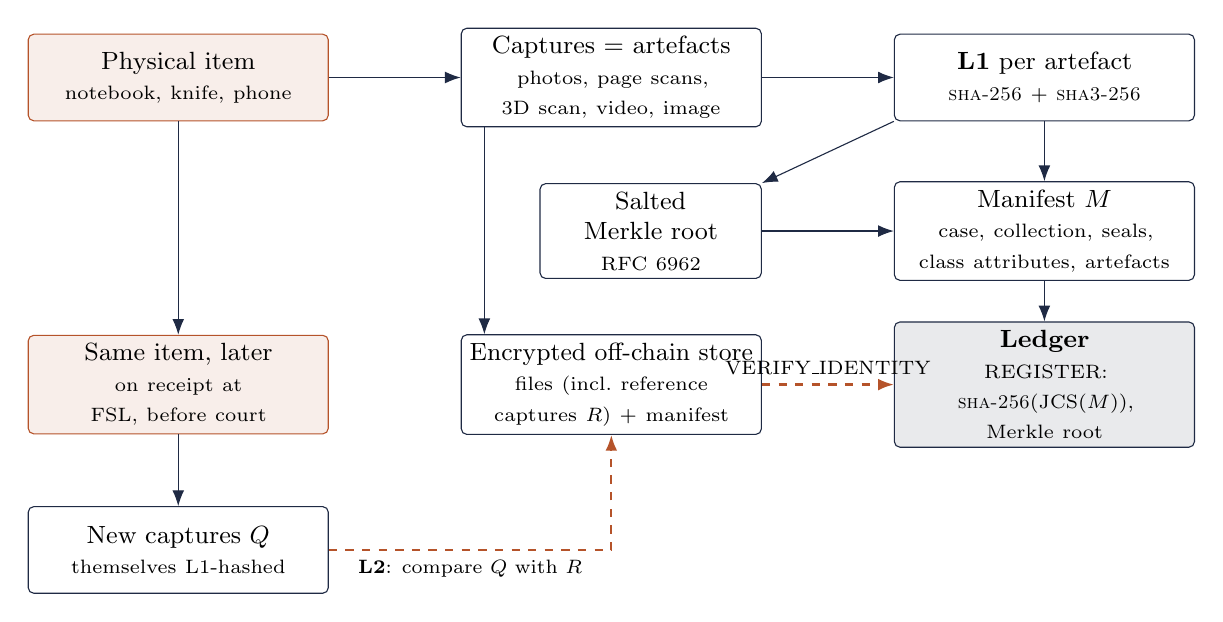
\begin{tikzpicture}[font=\small,
  box/.style={draw=ink, rounded corners=2pt, align=center, minimum height=11mm, text width=36mm, inner sep=3pt, fill=white},
  phys/.style={box, fill=accent!10, draw=accent},
  chain/.style={box, fill=ink!10},
  arr/.style={-{Latex[length=2mm]}, draw=ink},
  ltwo/.style={-{Latex[length=2mm]}, draw=accent, dashed, thick}]
  % column 1: the physical world
  \node[phys] (item)  at (0, 0)    {Physical item\\\scriptsize notebook, knife, phone};
  \node[phys] (later) at (0,-3.9)  {Same item, later\\\scriptsize on receipt at FSL, before court};
  \node[box]  (q)     at (0,-6.0)  {New captures $Q$\\\scriptsize themselves L1-hashed};
  % column 2: files
  \node[box]  (cap)   at (5.5, 0)  {Captures = artefacts\\\scriptsize photos, page scans, 3D scan, video, image};
  \node[box, text width=26mm] (mr) at (6.0,-1.95) {Salted Merkle root\\\scriptsize RFC 6962};
  \node[box]  (store) at (5.5,-3.9) {Encrypted off-chain store\\\scriptsize files (incl.\ reference captures $R$) + manifest};
  % column 3: integrity and ledger
  \node[box]  (l1)    at (11.0, 0)  {\textbf{L1} per artefact\\\scriptsize \shatwo{} + \shathree{}};
  \node[box]  (man)   at (11.0,-1.95) {Manifest $M$\\\scriptsize case, collection, seals, class attributes, artefacts};
  \node[chain](led)   at (11.0,-3.9) {\textbf{Ledger}\\\scriptsize REGISTER: $\shatwo(\mathrm{JCS}(M))$, Merkle root};
  % L1 path
  \draw[arr] (item) -- (cap);
  \draw[arr] (cap) -- (l1);
  \draw[arr] (l1) -- (man);
  \draw[arr] (l1.south west) -- (mr.north east);
  \draw[arr] (mr) -- (man);
  \draw[arr] (man) -- (led);
  \draw[arr] ([xshift=3mm]cap.south west) -- ([xshift=3mm]store.north west);
  % L2 path
  \draw[arr] (item) -- (later);
  \draw[arr] (later) -- (q);
  \draw[ltwo] (q.east) -| node[pos=0.25, below, font=\scriptsize, align=center]{\textbf{L2}: compare $Q$ with $R$} (store.south);
  \draw[ltwo] (store.east) -- node[above, font=\scriptsize]{VERIFY\_IDENTITY} (led.west);
\end{tikzpicture}
\caption{Data flow. Solid: Layer-1 integrity path from capture to ledger. Dashed: Layer-2 identity check of the same item later, whose result is itself recorded on the ledger.}
\label{fig:flow}
\end{figure}

\begin{table}[htbp]
\centering\small
\begin{tabularx}{\linewidth}{@{}lXX@{}}
\toprule
 & On-chain (every peer of the channel) & Off-chain (encrypted evidence store) \\
\midrule
Item & \code{evidence\_id}, class, parent id, \code{manifest\_sha256}, \code{merkle\_root}, artefact count, spec version & Full manifest (case facts, persons, locations, seals, attributes, per-artefact hashes and salts) \\
Files & nothing & All artefacts: originals (\enquote{master negative}) and working copies \\
Events & type, reason, references, seal readings, verification results, hashes of attachments; actor and time from the transaction & Attachments (receipts, FSL reports, orders) \\
Personal data & none in clear (witness names, addresses and accused details stay in the manifest) & manifest, access-controlled \\
\bottomrule
\end{tabularx}
\caption{What is stored where. Only fingerprints and custody metadata are replicated on the ledger (R7).}
\label{tab:onoff}
\end{table}

Verification by a third party (R8) needs only the file(s), the manifest and the ledger record:
\begin{enumerate}[nosep]
  \item recompute each artefact's \shatwo{}/\shathree{} and compare with the manifest;
  \item recompute the Merkle root \emph{from the files} and compare with the manifest;
  \item recompute $\shatwo(\mathrm{JCS}(M))$ and compare the manifest hash and root with the ledger record.
\end{enumerate}
If a single artefact must be disclosed without the rest (for example one page of a notebook), it is accompanied by its salt and an inclusion proof against the ledger's Merkle root (\cref{tab:proof}).

\subsection{The window of vulnerability}
\label{sec:window}
Integrity protection begins only when a hash is \emph{committed somewhere the adversary cannot change}. Two intervals matter: capture $\to$ first hash, and first hash $\to$ ledger anchoring. The design minimises both:
\begin{itemize}
  \item hash on the capture device immediately after capture. This is what the SOP's flowchart requires (\enquote{obtain hash value of A-V file}) and what e-Sakshya provides~\cite{sopbnss};
  \item record \code{hashed\_at} and \code{hashed\_on} for every artefact, so the window is visible to a court;
  \item when the device is offline, queue the hashes, sign them with the device or officer key, and submit them as soon as connectivity returns. The ledger timestamp then bounds the window from above;
  \item for removable media, follow the SOP: sealed envelope to the expert, hashed on opening in the presence of the officer, never opened in an editor before hashing~\cite{sopbnss}.
\end{itemize}

\section{Per-class fingerprinting procedures}
\label{sec:classes}

Each evidence class is specified below under the same headings. The complete list of mandatory and optional fields is in \cref{app:spec}; here we explain \emph{what is hashed and why}. The two classes raised in discussion, a crime-scene photograph and a recovered notebook, are treated first and in the most detail, because they show the contrast clearly. A photograph \emph{is} its file. A notebook is a physical object that can only be represented by files.

\newcommand{\cardrow}[2]{\textbf{#1} & #2 \\ \addlinespace[2pt]}
\newenvironment{classcard}{\par\smallskip\noindent\small\tabularx{\linewidth}{@{}>{\raggedright\arraybackslash}p{2.7cm}X@{}}\toprule}{\bottomrule\endtabularx\par\medskip}

% ---------------------------------------------------------------------------------------
\subsection{Crime-scene photograph (\code{SCENE\_PHOTOGRAPH})}
\label{sec:cls-photo}
A digital photograph is born-digital: the file produced by the camera is the primary evidence, and nothing needs to be \enquote{fingerprinted from the real world}. The exact bytes are hashed.

\begin{classcard}
\cardrow{Unit of record}{One photograph = one evidence item (frame), grouped by \code{photo\_series\_id}. The series follows the SOP's general-to-specific sequence: overall, mid-range and close-up views, with scale~\cite{sopbnss}.}
\cardrow{Mandatory inputs}{Case, collection (time, GNSS position, photographer, witnesses, legal basis), \code{view}, \code{frame\_number}, \code{scale\_present}, subject, original format, capture device with clock check.}
\cardrow{Artefacts}{The original file exactly as written by the device (JPEG/HEIC/RAW, EXIF intact).}
\cardrow{L1 (what is hashed)}{The \emph{entire original file}, pixels \emph{and} metadata, on the device immediately after capture. Hashing the file, rather than decoded pixels, means a change to the EXIF capture time is detected as well (\cref{tab:photo}).}
\cardrow{L2}{pHash of the image, used to recognise the same content when it resurfaces as a re-encoded copy, screenshot or print scan, and to detect a near-duplicate presented as a different photograph. Never used for integrity.}
\cardrow{Derived artefacts}{Any enhancement (crop, brightness, enlargement) is a \emph{new} artefact with \code{parent\_artefact\_id} set and its own hashes; the original stays in the manifest. The SOP requires enhancements to be documented and stored separately~\cite{sopbnss}.}
\cardrow{Pitfalls}{Opening the file in an editor or gallery app that rewrites metadata; messaging apps that recompress; deleting \enquote{bad} frames (the SOP forbids deleting photographically faulty images, which also keeps frame numbering continuous); an unsynchronised device clock (record \code{clock\_check}).}
\end{classcard}

\paragraph{Optional strengthening.} Capture applications that sign the image and its metadata at capture with a device key (for example under the C2PA content-credential specification~\cite{c2pa}) shorten the window of \cref{sec:window} to zero and bind the image to a specific enrolled device. This complements L1 and does not replace it.

% ---------------------------------------------------------------------------------------
\subsection{Recovered notebook or other physical document (\code{PHYSICAL\_DOCUMENT})}
\label{sec:cls-notebook}
A notebook cannot be hashed. Its integrity and identity rest on a \emph{reference capture set} made at seizure (or, at the latest, before it leaves the first custodian) and on the seal.

\begin{classcard}
\cardrow{Unit of record}{One document = one item. Each \emph{side} that is scanned is one \code{page\_scan} artefact with \code{sequence} = page number; cover and edge photographs are additional artefacts.}
\cardrow{Mandatory inputs}{Document type, \code{page\_count}, leaf count, dimensions, binding, writing media, \code{distinguishing\_features} (at least one), scan resolution ($\ge$ 300 dpi) and colour mode, seal and label identifiers.}
\cardrow{Artefacts}{(i) cover and edge photographs with scale; (ii) every side scanned flat at fixed dpi, \emph{lossless} PNG or TIFF, in page order, including blank sides; (iii) photograph of the sealed bag.}
\cardrow{L1 (what is hashed)}{Each scan file and photograph. The Merkle tree over the artefacts \emph{in page order} binds the ordered set: removing, inserting or substituting a page changes the root, and verification names the exact artefact (\cref{sec:worked}).}
\cardrow{L2}{(a) Seal number (exact) and seal-intact photograph at every transfer. (b) pHash of every page: on receipt at the FSL the pages are re-scanned and compared page by page. A substituted or re-written page fails, and a missing page shows up as a count mismatch and an unmatched reference. (c) Distinguishing features (tears, stains) on re-inspection.}
\cardrow{Limits}{Page-level pHash detects substitution and gross alteration of a page, but not a few added strokes or an altered digit. Such questions belong to questioned-document examination (ink, indentation, handwriting) by an expert, which the reference scans support but do not replace.}
\cardrow{Pitfalls}{Lossy JPEG scans (re-compression changes bytes and blurs fine detail); auto-deskew or \enquote{enhance} options of scanner software (disable them and record the settings); scanning only pages that look relevant.}
\end{classcard}

\begin{keypoint}[Photograph vs.\ notebook in one line]
For the photograph, \emph{the file is the evidence} and L1 alone answers the integrity question. For the notebook, \emph{the files represent the evidence}: L1 freezes the representation, and L2 plus the seal links the physical notebook to it at each later stage.
\end{keypoint}

% ---------------------------------------------------------------------------------------
\subsection{Search, seizure and statement recordings (\code{AV\_RECORDING})}
\begin{classcard}
\cardrow{Legal context}{Mandatory for search and seizure (BNSS s.105, s.185(2)) and, once notified, for scene-of-crime processing in offences punishable with seven years or more (s.176(3)); optional or conditional for statements~\cite{bnss2023,sopbnss}.}
\cardrow{Mandatory inputs}{Purpose, legal provision, start and end time, \code{media\_blank\_confirmed}, segment $n$ of $m$, codec, time forwarded to the Magistrate.}
\cardrow{L1}{Each segment file as written by the recorder, hashed on the device (or on first opening of the sealed card in the expert's presence). For long recordings, a \code{chunk\_merkle\_root} over fixed-size chunks localises any later corruption to a few seconds of footage.}
\cardrow{Continuity}{The SOP requires recording without breaks; when a card is changed, the change is filmed by a second recorder. Each segment is a separate artefact with \code{sequence}, and \code{continuity\_device\_ref} points to the second recorder's item.}
\cardrow{Copies for court}{The SOP's \enquote{master negative} and \enquote{mirror image} are byte copies, so their hashes \emph{equal} the original's. Equality of hashes is the proof that the copy produced is the recording made~\cite{sopbnss}.}
\end{classcard}

% ---------------------------------------------------------------------------------------
\subsection{CCTV export (\code{CCTV\_EXPORT})}
\begin{classcard}
\cardrow{Mandatory inputs}{System make, model and serial number; owner or operator (who signs Part A of the s.63 certificate); camera IDs; footage start and end; \code{dvr\_clock\_offset\_seconds}; export method.}
\cardrow{Artefacts}{The export file(s) in native format, the vendor's player (if proprietary), the export log, and a photograph of the DVR clock next to a reference clock.}
\cardrow{L1}{Every exported file and the player binary, hashed at the moment of export on the export medium.}
\cardrow{Notes}{DVR clocks are often wrong by minutes; the measured offset is recorded, not \enquote{corrected} in the file. Transcoding to MP4 for viewing creates a derived artefact; the native export remains the reference.}
\end{classcard}

% ---------------------------------------------------------------------------------------
\subsection{General physical item (\code{PHYSICAL\_ITEM})}
\begin{classcard}
\cardrow{Mandatory inputs}{Item category, dimensions, material, at least one unique mark, 3D-scan method, point spacing and stated accuracy (or the reason it was not performed), mass where measurable, expected changes (e.g.\ swabbing).}
\cardrow{Artefacts}{Photographs in a defined set of views with scale and colour reference; close-ups of unique marks; a 3D scan (structured light, laser or photogrammetry) exported as a mesh or point cloud in millimetres; a measurement record.}
\cardrow{L1}{Every photograph, the 3D-scan file and the measurement record.}
\cardrow{L2}{Seal number (exact); 3D deviation after ICP alignment (symmetric RMS and maximum against declared thresholds); serial numbers and unique marks; mass within instrument tolerance.}
\cardrow{Why 3D}{A photograph fixes appearance from one viewpoint; a 3D scan fixes geometry independently of viewpoint and lighting, so damage, substitution by a look-alike, or material removal can be measured (\cref{tab:knife}).}
\cardrow{Expected change}{Forensic tests legitimately alter items (swabbing, test-firing, sectioning). Each such step is an \code{EXAMINE} event; a new reference capture is taken afterwards and registered as a \code{DERIVE}d state, so later comparisons are made against the right reference.}
\end{classcard}

% ---------------------------------------------------------------------------------------
\subsection{Biological and trace samples (\code{BIO\_TRACE\_SAMPLE})}
\begin{classcard}
\cardrow{Specific problem}{The sample itself is consumed or changed by analysis and cannot be re-identified by its appearance. Its identity is carried by its \emph{container}.}
\cardrow{Mandatory inputs}{Sample type, collection method, container type, \code{container\_barcode}, quantity, storage condition (and temperature-log reference), biohazard flag.}
\cardrow{Artefacts}{Photographs of the sample in situ and of the sealed, labelled container; the temperature log for cold-chain items; laboratory reports.}
\cardrow{L1}{Photographs, temperature log, reports.}
\cardrow{L2}{Barcode and seal exact match, seal-intact photograph on receipt. Splitting into aliquots creates child items (\code{DERIVE}) with their own barcodes.}
\end{classcard}

% ---------------------------------------------------------------------------------------
\subsection{Seized digital device (\code{DIGITAL\_DEVICE})}
\begin{classcard}
\cardrow{Mandatory inputs}{The device fields of the BSA Schedule certificate (device type, make and model, colour, serial number, IMEI/UIN/UID/MAC); power state at seizure; isolation (Faraday bag, airplane mode); lock status. The credential itself is never stored in the manifest.}
\cardrow{Artefacts}{Photographs of the device and its screen state and labels; the seizure A/V reference.}
\cardrow{L1/L2}{The device is a physical item: L1 covers its photographs and L2 its serial and IMEI (exact) plus the seal. Its \emph{data} is fingerprinted separately when it is acquired (next two classes).}
\end{classcard}

% ---------------------------------------------------------------------------------------
\subsection{Forensic image of storage media (\code{FORENSIC\_IMAGE})}
\begin{classcard}
\cardrow{Mandatory inputs}{Parent device (\code{parent\_evidence\_id}), acquisition tool and exact version, write blocker (make, model, serial), image format, source size, \code{source\_stream\_sha256}, \code{verification\_sha256}, start and end, examiner.}
\cardrow{L1}{Two distinct hashes must agree: the \shatwo{} of the bit stream \emph{read from the source} during acquisition, and the \shatwo{} recomputed from the finished image. Container files (E01 segments, AFF4) are additionally hashed as artefacts. Tool-embedded \textsc{md5}/\textsc{sha-1} values are kept for cross-reference only.}
\cardrow{Notes}{Solid-state media with TRIM, wear levelling or live systems may never reproduce the same source hash on re-acquisition. The image, not the device, is then the integrity anchor, which is why the acquisition-time hash must be committed immediately. Chunk-level hashes localise later corruption of working copies (\cref{tab:disk}).}
\end{classcard}

% ---------------------------------------------------------------------------------------
\subsection{Mobile extraction (\code{MOBILE\_EXTRACTION})}
\begin{classcard}
\cardrow{Mandatory inputs}{Parent device, tool and version, extraction type (logical, file system, full file system, physical), device state, start and end, examiner.}
\cardrow{L1}{The extraction package and the tool's report, as produced. A phone is a live system: a second extraction will \emph{never} hash identically, so the hashes anchor this extraction, not the phone.}
\end{classcard}

% ---------------------------------------------------------------------------------------
\subsection{Cloud and social-media data (\code{CLOUD\_DATA})}
\begin{classcard}
\cardrow{Mandatory inputs}{Provider, account identifiers, legal process reference, date range, time of receipt, delivery method, provider-supplied hash or signature if any, capture format.}
\cardrow{L1}{The package exactly as received, hashed on receipt; any provider hash is recorded and checked. Web captures should be preserved as WARC with capture time rather than as screenshots.}
\cardrow{Notes}{Part A of the s.63 certificate for such data concerns the provider's systems; the record of exactly what was received, and when, is what this system can guarantee.}
\end{classcard}

% ---------------------------------------------------------------------------------------
\subsection{IoT and system logs (\code{IOT\_LOG})}
\begin{classcard}
\cardrow{Mandatory inputs}{Source system, device IDs, log start and end, time-synchronisation status, at-source integrity (hash-chained, signed, append-only store, none), export method, format.}
\cardrow{L1}{The exported log files. If the source hash-chains or signs its entries, the chain head is recorded so that completeness, not just integrity, of the export can be checked. Edge-side collection with on-chain anchoring, as in Chain4ensic~\cite{pezzoni2025}, reduces the window further.}
\end{classcard}

% ---------------------------------------------------------------------------------------
\subsection{Procedural documents (\code{PROCEDURAL\_DOCUMENT})}
\begin{classcard}
\cardrow{Scope}{Seizure memo, panchnama, chain-of-custody form, forwarding letter, FSL request and report, BSA s.63 certificate (Parts A and B), case-diary extracts, court orders.}
\cardrow{L1}{Born-digital PDFs: the file, preferably carrying an electronic signature under the IT Act~\cite{itact2000}. Paper: scanned exactly like a physical document (lossless, all pages).}
\cardrow{Role}{These documents tie the procedure to the evidence. Each item's manifest references the seizure memo (\code{seizure\_memo\_ref}) and each document references the items it covers (\code{refers\_to\_evidence\_ids}), so the cross-references are themselves hash-protected.}
\end{classcard}

\section{Lifecycle events}
\label{sec:lifecycle}

After registration, everything that happens to an item is an append-only \emph{custody event} (schema \code{custody-event.schema.json}). Events are never updated or deleted. A mistake is corrected by a \code{CORRECTION} event that references the erroneous one (R5). For every event the chaincode takes the \emph{who} (certificate subject and MSP) and the \emph{when} (transaction timestamp) from the transaction itself (R4). The client supplies only the \emph{what}, \emph{why}, \emph{where} and supporting references, which replaces the free-text 5W1H fields of the original prototype~\cite{loffi2025}.

\begin{table}[htbp]
\centering\small
\begin{tabularx}{\linewidth}{@{}lXl@{}}
\toprule
Event & Meaning and mandatory content & Allowed actor (proposed) \\
\midrule
\code{REGISTER} & Item enters the system; \code{manifest\_sha256}, \code{merkle\_root} & collecting officer \\
\code{SEAL} / \code{RESEAL} & Package sealed or resealed; seal IDs observed & current custodian \\
\code{TRANSFER\_INITIATE} & Custodian proposes a handover; receiving MSP and custodian & current custodian only \\
\code{TRANSFER\_ACCEPT} / \code{\_REJECT} & Receiver confirms or refuses; seal IDs read and \code{seal\_intact} & named receiver only \\
\code{ACCESS} & Item or files viewed without change & any authorised user \\
\code{EXAMINE\_START} / \code{\_END} & Examination opened or closed; attachments (lab notes, report hashes) & custodian (examiner) \\
\code{DERIVE} & Child item created (forensic image, extraction, aliquot, enhanced copy, post-test reference); child manifest hash & custodian \\
\code{VERIFY\_INTEGRITY} & L1 re-check: method, result, recomputed hashes & any authorised user \\
\code{VERIFY\_IDENTITY} & L2 re-identification: method, version, score, threshold, result, L1 hashes of the new captures & custodian \\
\code{SUBMIT\_COURT} & Produced before court; certificate hashes & custodian \\
\code{RETURN} / \code{ARCHIVE} / \code{DISPOSE} & End of lifecycle; court-order reference required & custodian (on order) \\
\code{CORRECTION} & Corrects an earlier event (by tx id) & author of the original event or supervisor \\
\bottomrule
\end{tabularx}
\caption{Custody event types. Custody passes only through the two-phase INITIATE/ACCEPT pair, so neither party can create a handover the other did not sign.}
\label{tab:events}
\end{table}

\paragraph{Two-phase transfer.} In the original prototype any client could set a new owner. Here, a transfer is proposed by the current custodian (checked against the certificate of the last accepted holder) and becomes effective only when the named receiver signs \code{TRANSFER\_ACCEPT}. The receiver records the seal numbers read and whether the seal is intact. A broken seal does not block the transfer, since evidence must still move, but it is permanently recorded and should trigger a \code{VERIFY\_IDENTITY}.

\paragraph{Example timeline for the notebook (item E004).}
\begin{enumerate}[nosep]
  \item \code{REGISTER} by the IO at the scene: 2 photographs and 6 page scans, Merkle root over 8 leaves (\cref{tab:nbled}).
  \item \code{SEAL}: bag \code{TEB-GJ-0007741}.
  \item \code{TRANSFER\_INITIATE} to \code{FSLMSP}, with the forwarding-letter reference as reason.
  \item \code{TRANSFER\_ACCEPT} at the FSL counter: seal read, intact.
  \item \code{VERIFY\_IDENTITY}: re-scan of 6 sides, maximum pHash distance \NbRescanMaxDist{} $\le 10$, MATCH (\cref{tab:nbrescan}).
  \item \code{EXAMINE\_START} \ldots{} \code{EXAMINE\_END}, with the hash of the FSL report attached.
  \item \code{TRANSFER\_INITIATE} and \code{\_ACCEPT} back to the police, then \code{SUBMIT\_COURT}, with the hashes of the s.63 certificates attached.
\end{enumerate}
The example events are in \code{spec/examples/notebook.events.json} and validate against the schema.

\paragraph{From events to the paper chain-of-custody form.} The SOP requires, for every package, the name and signature of each person who takes possession of or transports the evidence, the date of transfer and the evidence label or serial number, recorded chronologically and without opinion~\cite{sopbnss}. Every one of these fields is present in the event history, with the signature replaced by the ledger-verified certificate signature. The form can therefore be printed from the ledger rather than maintained separately.

\section{Indian legal and procedural mapping}
\label{sec:legal}

The Bharatiya Nagarik Suraksha Sanhita (BNSS), Bharatiya Sakshya Adhiniyam (BSA) and Bharatiya Nyaya Sanhita (BNS) replaced the CrPC, the Indian Evidence Act and the IPC with effect from 1 July 2024~\cite{bnss2023,bsa2023,bns2023}. For this system the decisive change is that audio-video recording and hashing are now \emph{statutory procedure}, not merely good practice. This section is a technical mapping prepared from the statutes as summarised in the SOP for audio-visual recording~\cite{sopbnss} and from government statements~\cite{rs1332,pib2026}. It is not legal advice, and the points marked \emph{to verify} should be confirmed with a legal expert before the design is relied on.

\subsection{Provisions that shape the design}
\begin{table}[htbp]
\centering\small
\begin{tabularx}{\linewidth}{@{}>{\raggedright}p{2.6cm}X>{\raggedright\arraybackslash}p{4.4cm}@{}}
\toprule
Provision & Requirement (as summarised in~\cite{sopbnss}) & System support \\
\midrule
BNSS s.105 & Search and seizure, including preparing the list of seized things and its signing by witnesses, \emph{shall} be recorded by audio-video electronic means, preferably a mobile phone; the recording is forwarded without delay to the Magistrate. & \code{AV\_RECORDING} item referenced by every seized item (\code{av\_recording\_ref}); \code{forwarded\_to\_magistrate\_at}. \\
BNSS s.185(2) & A search by a police officer shall be recorded by audio-video means, preferably mobile phone. & As above. \\
BNSS s.176(3) & For offences punishable with 7 years or more, from a date notified by the State (within five years), a forensic expert visits the scene to collect forensic evidence, and the process is videographed. & \code{SCENE\_PHOTOGRAPH}, \code{AV\_RECORDING}, and the physical classes; the legal basis is recorded per item. \\
BNSS s.173, s.180, s.183(6)(a) & Video recording of information and statements in specified circumstances (mandatory for some victims or witnesses with disability). & \code{AV\_RECORDING} with \code{purpose} = statement. \\
BNSS s.497(3) & The court causes property pending trial to be photographed and, if necessary, videographed before custody or disposal. & \code{DISPOSE}/\code{RETURN} events require the court order and the hashes of the photographs. \\
BNSS s.193 & The SOP flowchart directs that the chain of custody be submitted with the charge-sheet. & Chain-of-custody form generated from events (\cref{sec:lifecycle}). \\
BNSS s.329 & Reports of notified Government scientific experts may be used as evidence. & FSL organisation and examiner identities; report hashes on \code{EXAMINE\_END}. \\
BSA s.61 & An electronic or digital record is not to be denied admissibility merely because it is electronic (subject to s.63). & Basis for treating hashed digital captures as evidence. \\
BSA s.57, s.58 & Primary vs.\ secondary evidence; explanations address electronic records. & Originals (master negative) vs.\ copies: copies are proven by \emph{equal hashes}. \\
BSA s.63(4)(c) and the Schedule & A certificate accompanies the electronic record \emph{at each instance} it is submitted. Part~A is completed by the person in charge of the device or activity, Part~B by an expert. Both state the device details and \textbf{the hash value(s) and algorithm} (SHA1, SHA256, MD5 or another legally acceptable standard), with the hash report enclosed. & \Cref{tab:bsa}: every field is in the manifest; certificates are themselves \code{PROCEDURAL\_DOCUMENT} items. \\
BSA s.39(2); IT Act s.79A & The opinion of a notified Examiner of Electronic Evidence is a relevant fact. & Examiner identity on FSL events. \\
\bottomrule
\end{tabularx}
\caption{Statutory provisions and how the design supports them.}
\label{tab:law}
\end{table}

\subsection{The Section 63 certificate as a data model}
The Schedule certificate~\cite{bsa2023} (reproduced in~\cite{sopbnss}) fixes the information that must accompany any electronic record. The manifest captures every field, so Parts~A and~B can be generated directly from it (R9):

\begin{table}[htbp]
\centering\small
\begin{tabularx}{\linewidth}{@{}>{\raggedright}p{0.40\linewidth}>{\raggedright\arraybackslash}X@{}}
\toprule
Schedule field (Parts A and B) & Manifest source \\
\midrule
Device or record source (Computer/Storage Media, DVR, Mobile, Flash Drive, CD/DVD, Server, Cloud, Other) & \code{capture\_device.device\_type} / \code{class\_attributes.device\_type} (same enumeration) \\
Make and model, colour, serial number & \code{capture\_device.make\_model}, \code{colour}, \code{serial\_number} \\
IMEI / UIN / UID / MAC / Cloud ID & \code{capture\_device.imei\_uin\_uid\_mac\_cloud\_id} \\
Owned / maintained / managed / operated by the certifier & \code{collection.collected\_by} or the CCTV \code{owner\_or\_operator} \\
Hash value(s) and algorithm; hash report enclosed & \code{artefacts[].sha256} (algorithm SHA256) and \code{sha3\_256} (\enquote{Other}); the hash report is the manifest itself \\
Date, time (IST, 24 h), place & \code{hashed\_at}, \code{location} \\
Name, designation, signature (Part B: expert) & \code{person} records and the certificate signature on the ledger \\
\bottomrule
\end{tabularx}
\caption{BSA Schedule certificate fields mapped to the manifest.}
\label{tab:bsa}
\end{table}

\begin{caution}[MD5 and SHA-1 on the statutory form]
The Schedule offers MD5 and SHA-1 as options. Both are cryptographically broken for collision resistance~\cite{wang2005,stevens2017}. The system should always certify SHA-256, adding SHA3-256 under \enquote{Other}, and treat MD5/SHA-1 values produced by legacy tools only as cross-references.
\end{caution}

\subsection{Master negative, mirror image and the ledger}
The SOP describes the procedure the design implements~\cite{sopbnss}:
\begin{itemize}
  \item the first responder hashes the recording on the device (or the sealed card is opened and hashed by the expert in the officer's presence) and gives a Part~A certificate;
  \item the expert copies it to a designated disk, the \enquote{master negative}, which is never altered;
  \item the expert re-hashes and confirms the hashes match, gives Part~B, and produces a \enquote{mirror image} copy for the Magistrate;
  \item backups of the master negative are kept at a second location, \enquote{maybe for decades};
  \item hash values are entered in the case diary.
\end{itemize}

In this design the master negative is the off-chain evidence store, and the ledger is the tamper-evident, multi-agency \emph{case diary of hashes}:
\begin{itemize}
  \item every hash comparison in the SOP becomes a \code{VERIFY\_INTEGRITY} event;
  \item every handover becomes a two-phase transfer;
  \item the hash written in the case diary becomes an anchored manifest hash that no single agency can alter.
\end{itemize}

\subsection{Government systems}
The Ministry of Home Affairs has launched \textbf{e-Sakshya} for capturing, storing and retrieving evidence by photography and videography and for recording witness statements. As of February 2026 it was in use in 15{,}899 police stations across 35 States/UTs~\cite{rs1332}. It is described as creating a secure ecosystem for primary digital evidence and \enquote{ensuring integrity and authenticity of primary evidence from collection to presentation in court}~\cite{pib2026}. The SOP notes that NIC has developed it to capture audio/video and \enquote{generate hash reports with time stamps}~\cite{sopbnss}. The Interoperable Criminal Justice System (ICJS) exchanges records between police, courts, prisons, forensics and prosecution, and e-Forensic manages cases across forensic laboratories~\cite{pib2026}.

\begin{keypoint}[Positioning]
CustodyChain does not compete with e-Sakshya or ICJS. Its contribution is a \emph{multi-agency, append-only commitment layer} beneath them. Hashes produced by e-Sakshya at capture, events from e-Forensic and charge-sheet records from ICJS can all be anchored so that no single operator, the system owner included, can silently rewrite them. The integration interface is the manifest and the event schema.
\end{keypoint}

\subsection{Other legal considerations}
\begin{itemize}
  \item \textbf{Electronic signatures.} Procedural documents can carry electronic signatures under the IT Act 2000~\cite{itact2000}; ledger signatures are certificate-based but are not, by themselves, IT-Act electronic signatures. \emph{To verify:} whether ledger certificate signatures need to be issued under a licensed Certifying Authority to carry statutory weight.
  \item \textbf{Personal data.} Manifests contain personal data (witnesses, accused, victims). The Digital Personal Data Protection Act 2023~\cite{dpdp2023} contains exemptions for the prevention, detection, investigation and prosecution of offences, but retention and erasure policies still have to be defined. Keeping personal data only in the off-chain manifest (\cref{tab:onoff}), with salted leaves on-chain, means an off-chain record can be deleted or crypto-shredded under a court order while the ledger keeps only a commitment that reveals nothing. \emph{To verify:} the precise scope of the exemption.
  \item \textbf{Seizure of electronic devices.} The SOP records that, pending guidelines in \emph{Ram Ramaswamy v.\ Union of India}, the Supreme Court has directed central agencies to follow the CBI manual in the interim~\cite{sopbnss}. Procedures for the digital classes should be aligned with it.
\end{itemize}

\section{The network: consensus, organisations and persistence}
\label{sec:network}

\subsection{Where consensus happens in Hyperledger Fabric}
Fabric uses an \emph{execute--order--validate} architecture~\cite{androulaki2018}:
\begin{enumerate}[nosep]
  \item \textbf{Execute.} The client sends a proposal to endorsing peers. Each peer simulates the chaincode and signs the result (the read/write set). The endorsement policy decides whose signatures are required.
  \item \textbf{Order.} The client sends the endorsed transaction to the \emph{ordering service}, which agrees on a single total order of transactions and cuts blocks.
  \item \textbf{Validate.} Every peer checks each transaction's endorsements against the policy and checks for conflicts, then appends the block to its ledger.
\end{enumerate}
\emph{Consensus} in the classical sense, agreement among nodes on the order of history, is the job of the ordering nodes (orderers). Peers do not vote on order. When the requirement is \enquote{at least four consensus nodes}, it therefore refers to \textbf{orderers}.

\subsection{Kafka, Raft and BFT}
\begin{description}[style=nextline,leftmargin=1.2em]
  \item[Kafka (not used).] Early Fabric releases ordered transactions through an Apache Kafka/ZooKeeper cluster. Kafka-based ordering was deprecated in Fabric v2, and \enquote{since release V3.0 Solo, Kafka and the System Channel have been removed} (Fabric 3.1.5 sample configuration). The current network does \emph{not} use Kafka: its channel configuration declares \code{OrdererType: etcdraft} (Raft).
  \item[Raft (current, crash fault tolerant).] A leader-based protocol~\cite{ongaro2014}. With $n$ orderers it tolerates $f$ \emph{crashed} nodes if $n \ge 2f+1$, but it assumes no node lies: a compromised leader could, for example, censor transactions. The test network inherited from the paper runs \textbf{a single} Raft orderer, so it has no fault tolerance and no consensus among independent parties in any meaningful sense.
  \item[BFT (decided).] Byzantine fault tolerance~\cite{lamport1982,castro1999} tolerates nodes that crash \emph{or behave arbitrarily}: send conflicting messages, propose invalid blocks, or collude. Fabric v3 ships a BFT ordering service based on the SmartBFT library~\cite{barger2021,fabricdocs}.
\end{description}

\paragraph{Why four is the minimum.} BFT protocols in the PBFT family need $n \ge 3f+1$ nodes to tolerate $f$ Byzantine nodes, and decisions require a quorum of $2f+1$. The intuition: a node can wait for only $n-f$ replies, because $f$ may never answer. Of those replies, up to $f$ may be lies, so the honest replies ($n-2f$) must still outnumber the lies ($f$), which requires $n-2f > f$, i.e.\ $n > 3f$. With $f=1$: $n=4$ and quorum $3$.

\begin{table}[htbp]
\centering\small
\begin{tabular}{@{}>{\centering}p{1.6cm}>{\centering}p{2.3cm}>{\centering}p{2.6cm}>{\centering}p{1.5cm}l@{}}
\toprule
Orderers $n$ & Raft: crashes tolerated & BFT: faulty nodes tolerated & BFT quorum & Comment \\
\midrule
1 & 0 & -- & -- & current test network \\
3 & 1 & 0 & -- & Raft minimum for fault tolerance \\
\textbf{4} & 1 & \textbf{1} & \textbf{3} & \textbf{BFT minimum; implemented} \\
7 & 3 & 2 & 5 & \\
10 & 4 & 3 & 7 & \\
\bottomrule
\end{tabular}
\caption{Fault tolerance by number of ordering nodes.}
\end{table}

\subsection{Organisations}
To make \enquote{no single agency can rewrite history} (R6) concrete, each consensus node is operated by a different agency. In the test phase all of them run on one laptop.

\begin{figure}[htbp]
\centering
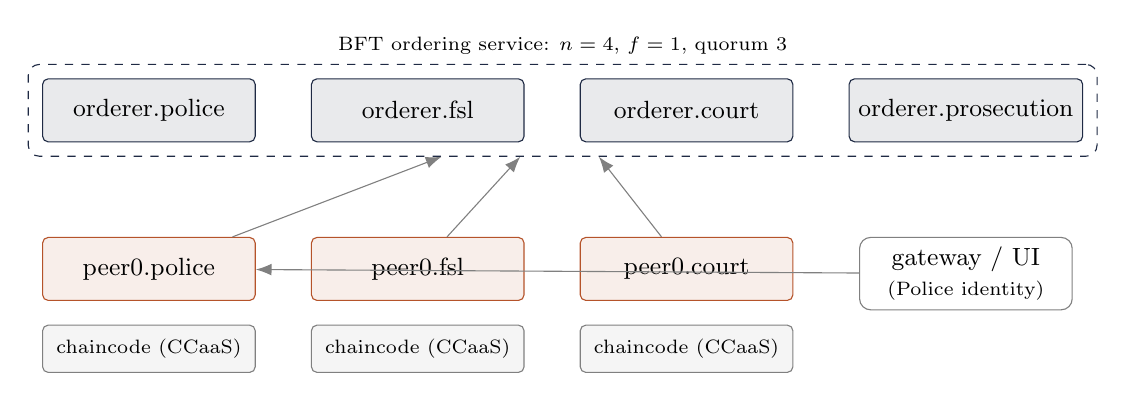
\begin{tikzpicture}[font=\small, node distance=5mm and 7mm,
  ord/.style={draw=ink, fill=ink!10, rounded corners=2pt, minimum width=27mm, minimum height=8mm, align=center},
  peer/.style={draw=accent, fill=accent!10, rounded corners=2pt, minimum width=27mm, minimum height=8mm, align=center},
  cc/.style={draw=gray, fill=gray!8, rounded corners=2pt, minimum width=27mm, minimum height=6mm, align=center, font=\scriptsize}]
  \node[ord] (o1) {orderer.police};
  \node[ord, right=of o1] (o2) {orderer.fsl};
  \node[ord, right=of o2] (o3) {orderer.court};
  \node[ord, right=of o3] (o4) {orderer.prosecution};
  \node[draw=ink, dashed, rounded corners, fit=(o1)(o4), inner sep=5pt, label={[font=\scriptsize]above:BFT ordering service: $n=4$, $f=1$, quorum 3}] (os) {};
  \node[peer, below=12mm of o1] (p1) {peer0.police};
  \node[peer, below=12mm of o2] (p2) {peer0.fsl};
  \node[peer, below=12mm of o3] (p3) {peer0.court};
  \node[cc, below=3mm of p1] {chaincode (CCaaS)};
  \node[cc, below=3mm of p2] {chaincode (CCaaS)};
  \node[cc, below=3mm of p3] {chaincode (CCaaS)};
  \node[draw=gray, rounded corners, minimum width=27mm, minimum height=8mm, below=12mm of o4, align=center] (gw) {gateway / UI\\\scriptsize (Police identity)};
  \foreach \p in {p1,p2,p3} \draw[-{Latex[length=2mm]}, gray] (\p) -- (os);
  \draw[-{Latex[length=2mm]}, gray] (gw) -- (p1);
\end{tikzpicture}
\caption{Implemented test topology: four agency-operated BFT orderers and three agency peers on channel \code{custody}.}
\label{fig:topology}
\end{figure}

\paragraph{What this buys and what it does not.} With one faulty or malicious orderer, say a compromised Police node, the remaining three still form a quorum and the ledger keeps progressing correctly; the faulty node can neither reorder nor forge blocks. If two of the four are faulty, BFT can no longer guarantee progress. Endorsement policies add a second, independent control. For example, requiring the endorsement of both the sending and the receiving agency for transfers means no single agency's peer can fabricate a handover. BFT does \emph{not} make data entered at collection true, and it cannot stop collusion of a quorum.

\paragraph{Peer count.} BFT governs orderers only. Peers hold ledger copies and endorse, and three (one per agency that handles evidence) are enough to demonstrate multi-agency endorsement. The architecture scales to more peers and orderers when hardware allows.

\subsection{Persistence}
\label{sec:persistence}
In the inherited scripts, \code{network.sh down} was the only way to stop the network, and it deletes the ledger volumes, the world state and all certificates. This is why every hash and every history disappeared between sessions. This has been fixed:
\begin{itemize}
  \item \code{network.sh stop} stops all Fabric containers (chaincode, peers, orderers, CAs) and deletes nothing;
  \item \code{network.sh start} resumes them from their persisted Docker volumes, in dependency order;
  \item \code{network.sh down} remains, explicitly, the \enquote{wipe everything} command, and now warns accordingly.
\end{itemize}
The chaincode containers are no longer started with \code{--rm}, so they survive a stop, and they carry the Fabric label so the lifecycle commands find them.

\paragraph{Tests performed (19 Nov 2026, Raft test network).} Each test started from a fresh network with one record:
\begin{enumerate}[nosep]
  \item record created, giving height 7 and current block hash \code{ypZfn9Vp...};
  \item \code{stop} and \code{start}: the height and hash were identical, the record was intact, and a new write committed as block 8;
  \item all containers killed with \code{docker kill} to simulate power loss, then \code{start}: both peers came back at height 8 with identical hashes and both records.
\end{enumerate}
A reboot of the host is equivalent to case 3: containers are left stopped with their volumes intact.

\subsection{Implementation status}
\label{sec:netstatus}
The BFT network of \cref{fig:topology} is implemented in \code{CustodyChain/backend/network-bft/} on Hyperledger Fabric v3.1.5 (SmartBFT ordering), and runs on the test laptop next to the paper's original Raft network, which is kept for reproduction. \code{test-bft.sh} verifies it end to end. The results of the run on 19~November~2026, on a freshly created network, are below.

\begin{table}[htbp]
\centering\small
\begin{tabularx}{\linewidth}{@{}c>{\raggedright}p{4.6cm}X@{}}
\toprule
\# & Test & Result \\
\midrule
1 & Channel configuration & \code{ConsensusType: BFT}; 4 consenters (IDs 1--4: Police, FSL, Court and Prosecution orderer MSPs). PASS \\
2 & Transaction, all orderers up & Committed VALID on all three peers in 0.2~s. The block carries \textbf{3 consenter signatures} (consenters 1, 2, 4), i.e.\ it is certified by a BFT quorum rather than a single orderer. PASS \\
3 & One orderer stopped ($f=1$) & Committed with 3 of 4 orderers in 0.2~s. PASS \\
4 & Two orderers stopped (no quorum) & No block produced; ledger height unchanged. BFT stops rather than risk safety. The pending request was not lost: it was ordered once the quorum returned. PASS \\
5 & Recovery & Commits resumed about 56~s after the two orderers restarted; all four orderers caught up to the same height. PASS \\
6 & Leader failure & The current leader (consenter 2, FSL) was stopped; a view change elected consenter 3 and commits resumed after about 54~s, which is bounded by the configured SmartBFT timeouts. PASS \\
7 & Persistence & \code{stop}/\code{start}: identical heights, block hashes and world state; new writes commit. PASS \\
8 & Resource use & 10 containers (4 orderers, 3 peers, 3 chaincode services) use about 370~MiB of RAM in total. \\
\bottomrule
\end{tabularx}
\caption{Verification of the BFT network (\code{network-bft/test-bft.sh}).}
\label{tab:bfttests}
\end{table}

The web gateway of the original prototype was made configurable through environment variables (defaults unchanged) and works against the BFT network through the Police peer. The recovery and view-change times reflect the test configuration (\code{LeaderHeartbeatTimeout} 1~min, \code{ViewChangeTimeout} 20~s, request complaint timeout 20~s). They can be tuned, but faster failure detection increases spurious view changes. With about 370~MiB for the whole network, the laptop can comfortably run larger configurations, for example 7 orderers ($f=2$), if required. The Fabric v3 test images are designed for single-host testing; production would place each agency's nodes on its own infrastructure.

Blocks are accepted by peers only with signatures of 3 of the 4 consenters: for BFT channels Fabric 3.1.5 derives the \code{BlockValidation} policy from the consenter mapping automatically (verified in the deployed configuration; D-050, \cref{sec:eval}).


\section{Worked examples}
\label{sec:worked}

All values in this section were computed by \code{tools/make\_worked\_examples.py} using the reference tool \code{tools/evidence\_hash.py}. The evidence is synthetic but follows the procedures of \cref{sec:classes}. Salts are derived from a fixed demonstration seed so that the numbers are reproducible; in production they are random. The resulting manifests validate against the schema and are in \code{spec/examples/}.

\subsection{Crime-scene photograph: why integrity and identity are different questions}
\Cref{fig:scene} shows the reference photograph, a second photograph of the same scene taken seconds later, and a copy of the reference with the knife digitally removed. \Cref{tab:photo} compares seven variants with the reference by exact hash (L1) and by perceptual hash (L2).

\begin{figure}[htbp]
\centering
\begin{tabular}{ccc}
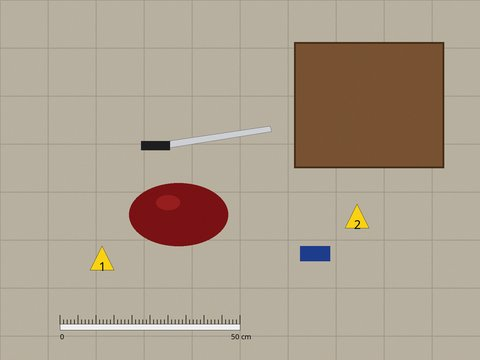
\includegraphics[width=0.31\linewidth]{figures/scene_original.jpg} &
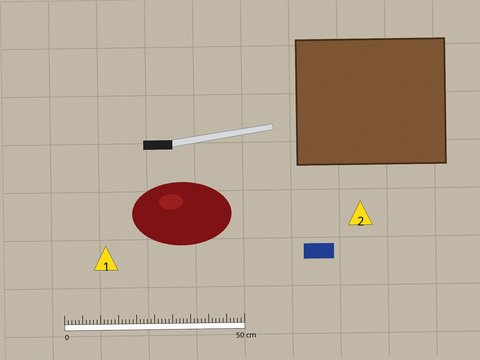
\includegraphics[width=0.31\linewidth]{figures/scene_second.jpg} &
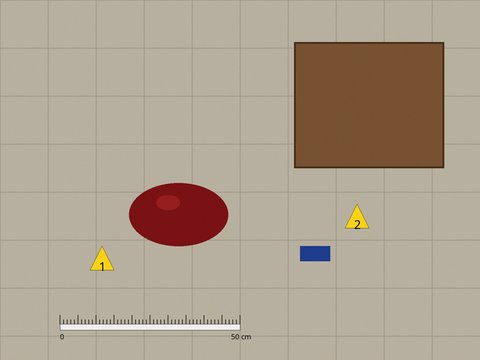
\includegraphics[width=0.31\linewidth]{figures/scene_tampered.jpg} \\
\small (a) reference \code{IMG\_0001} & \small (b) second shot, same scene & \small (c) knife digitally removed
\end{tabular}
\caption{Synthetic scene photographs (reduced).}
\label{fig:scene}
\end{figure}

\begin{table}[htbp]
\centering\small
\begin{tabular}{@{}p{0.30\linewidth}p{0.25\linewidth}cc>{\centering\arraybackslash}p{0.11\linewidth}@{}}
\toprule
Variant of \texttt{IMG\_0001} & SHA-256 (first 16 hex) & L1 equal? & pHash $d_H$ & L2 ($d_H\le 10$)\\
\midrule
Original file as produced by the device & \texttt{0ee55003\allowbreak{}4602fa2d\ldots} & yes & 0 & same\\
Byte-for-byte copy (e.g. to the master-negative disk) & \texttt{0ee55003\allowbreak{}4602fa2d\ldots} & yes & 0 & same\\
Opened and re-saved as JPEG (same quality setting) & \texttt{f769b244\allowbreak{}9ec51305\ldots} & \textbf{no} & 0 & same\\
Only the EXIF date/time edited; pixels untouched & \texttt{c5c6eeca\allowbreak{}12251f4f\ldots} & \textbf{no} & 0 & same\\
Second photograph of the same scene, seconds later & \texttt{81e30dfc\allowbreak{}25a89d1d\ldots} & \textbf{no} & 0 & same\\
Original with the knife digitally removed & \texttt{2e2864e3\allowbreak{}1f9b783b\ldots} & \textbf{no} & 0 & same\\
Photograph of a different scene & \texttt{90ed56c4\allowbreak{}0568ae5a\ldots} & \textbf{no} & 28 & different\\
\bottomrule
\end{tabular}

\caption{Seven variants of a scene photograph compared with the reference by \shatwo{} (L1) and 64-bit DCT pHash (L2).}
\label{tab:photo}
\end{table}

What the table shows:
\begin{itemize}
  \item \textbf{Only a byte-for-byte copy passes L1.} Re-saving with identical settings, or editing one EXIF field without touching a pixel, produces an unrelated \shatwo{}. This is why the SOP insists that recordings are never opened in editing software before hashing~\cite{sopbnss}.
  \item \textbf{A second photograph of the same scene} fails L1, as every new capture must (\enquote{no two photographs are the same}), yet is recognised by L2 (distance \PhotoSecondDist{}).
  \item \textbf{The tampered image passes L2} (distance \PhotoTamperDist{}) and is caught only by L1. Perceptual fingerprints must therefore never be used to establish integrity.
  \item \textbf{A different scene} is far away in L2 (distance \PhotoOtherDist{}).
\end{itemize}

\subsection{Recovered notebook: page scans, Merkle tree, tampering and re-identification}
The notebook (item E004) is documented by a cover photograph, an edge photograph and six lossless page scans at 300~dpi (\cref{fig:notebook}). \Cref{tab:nbart} lists the artefacts, and \cref{tab:nbled} shows what is written to the ledger.

\begin{figure}[htbp]
\centering
\begin{tabular}{cc}
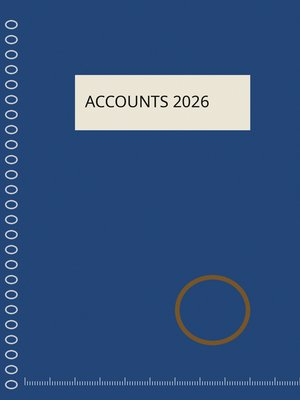
\includegraphics[height=5.2cm]{figures/notebook_cover.jpg} &
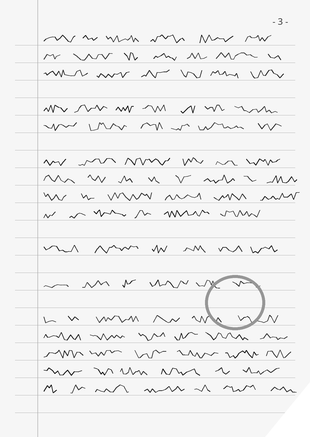
\includegraphics[height=5.2cm]{figures/notebook_page3.png} \\
\small cover photograph (A001) & \small page 3 scan (A005): torn corner, ring stain
\end{tabular}
\caption{Reference captures of the notebook (reduced).}
\label{fig:notebook}
\end{figure}

\begin{table}[htbp]
\centering\small
\begin{tabular}{@{}clll@{}}
\toprule
Artefact & Role & Size (bytes) & SHA-256\\
\midrule
\texttt{A001} & cover\_photo & 326615 & \texttt{fab9701b\allowbreak{}8a921d58\allowbreak{}38fc5c7e\ldots}\\
\texttt{A002} & edge\_photo & 128632 & \texttt{3dedfa67\allowbreak{}c8b545f3\allowbreak{}b0499be1\ldots}\\
\texttt{A003} & page\_scan & 38947 & \texttt{4b83b163\allowbreak{}6bb458bd\allowbreak{}4f1f8ba5\ldots}\\
\texttt{A004} & page\_scan & 41227 & \texttt{c71aed67\allowbreak{}a84ba93a\allowbreak{}6fcad3ab\ldots}\\
\texttt{A005} & page\_scan & 38765 & \texttt{6f56721a\allowbreak{}bffa9ba0\allowbreak{}c1d308ce\ldots}\\
\texttt{A006} & page\_scan & 36499 & \texttt{9d17cf12\allowbreak{}86e73ba1\allowbreak{}fc14b41d\ldots}\\
\texttt{A007} & page\_scan & 38053 & \texttt{76eb8499\allowbreak{}bda3742a\allowbreak{}ac892885\ldots}\\
\texttt{A008} & page\_scan & 43709 & \texttt{b074bdfa\allowbreak{}579c82af\allowbreak{}ca8858cd\ldots}\\
\bottomrule
\end{tabular}

\caption{Notebook artefacts in Merkle-leaf order (SHA-256 truncated).}
\label{tab:nbart}
\end{table}

\begin{table}[htbp]
\centering\small
\begin{tabular}{@{}lp{0.62\linewidth}@{}}
\toprule
Ledger field & Value\\
\midrule
\texttt{evidence\_id} & \texttt{GJ-GNR-CYBPS-2026-000123-E004}\\
\texttt{evidence\_class} & \texttt{PHYSICAL\_DOCUMENT}\\
\texttt{artefact\_count} & 8\\
\texttt{manifest\_sha256} & \texttt{d5b71925\allowbreak{}0e11dda2\allowbreak{}55782f9f\allowbreak{}a1d4b77d\allowbreak{}746ae94d\allowbreak{}7a5bc523\allowbreak{}2df470b2\allowbreak{}e902ade1}\\
\texttt{merkle\_root} & \texttt{6e845149\allowbreak{}4a032e33\allowbreak{}17bc66df\allowbreak{}35c259c9\allowbreak{}68a35e2f\allowbreak{}c67832d4\allowbreak{}f079695e\allowbreak{}9c514102}\\
\bottomrule
\end{tabular}

\caption{Ledger record of the notebook: the only data about E004 replicated on-chain.}
\label{tab:nbled}
\end{table}

\paragraph{Attack 1: a page is substituted in the evidence store.} An insider replaces the scan of page 4 with a scan of a re-written page 4. Verification against the manifest reports:
\begin{itemize}[nosep]
\item A006 (page\_004.png): size\_bytes mismatch: manifest 36499 != file 1140696
\item A006 (page\_004.png): sha256 mismatch: manifest \texttt{9d17cf1286e7\ldots} != file \texttt{2edd917f266b\ldots}
\item A006 (page\_004.png): sha3\_256 mismatch: manifest \texttt{08601e27fb44\ldots} != file \texttt{fef33dd0e7c5\ldots}
\item Merkle root from files mismatch: manifest \texttt{6e8451494a03\ldots} != files \texttt{d2e3ffa44a09\ldots}
\end{itemize}

The exact artefact (A006, page 4) is identified, and the Merkle root recomputed from the files no longer matches.

\paragraph{Attack 2: the insider also rewrites the manifest.} The manifest is now internally consistent with the forged page, but it no longer matches the ledger:
\begin{itemize}[nosep]
\item Manifest hash mismatch: ledger \texttt{d5b719250e11\ldots} != manifest \texttt{ffd436514d57\ldots}
\item Merkle root mismatch: ledger \texttt{6e8451494a03\ldots} != manifest \texttt{d2e3ffa44a09\ldots}
\end{itemize}

Defeating this would require changing the ledger record, which needs a BFT quorum of agencies (\cref{sec:network}).

\paragraph{Selective disclosure.} To show a court only page 4, the custodian discloses that page, its salt and the inclusion proof in \cref{tab:proof}. The verifier recomputes the leaf and the path and obtains the ledger's Merkle root without seeing any other page.

\begin{table}[htbp]
\centering\small
\begin{tabular}{@{}ll@{}}
\toprule
Leaf (artefact) & \texttt{A006} (page 4), index 5 of 8\\
Leaf salt & \texttt{3d4e9066\allowbreak{}c4cdde07\allowbreak{}f02e0b2a\allowbreak{}fee9a8e9\ldots}\\
Artefact SHA-256 & \texttt{9d17cf12\allowbreak{}86e73ba1\allowbreak{}fc14b41d\allowbreak{}ad74b931\ldots}\\
Audit path [0] & \texttt{f6406262\allowbreak{}fac99752\allowbreak{}72a7909c\allowbreak{}44f361d2\ldots}\\
Audit path [1] & \texttt{f554525c\allowbreak{}9214f3fe\allowbreak{}ee254972\allowbreak{}21aa3293\ldots}\\
Audit path [2] & \texttt{55fba80e\allowbreak{}03452a81\allowbreak{}83405fce\allowbreak{}cc05bb60\ldots}\\
Merkle root & \texttt{6e845149\allowbreak{}4a032e33\allowbreak{}17bc66df\allowbreak{}35c259c9\ldots}\\
Proof verifies & yes\\
\bottomrule
\end{tabular}

\caption{RFC 6962 inclusion proof for page 4 (hashes truncated). Three sibling hashes suffice for eight leaves.}
\label{tab:proof}
\end{table}

\paragraph{Re-identification at the FSL.} On receipt, all six sides are re-scanned on a different scanner. \Cref{tab:nbrescan} shows that every \shatwo{} differs, as expected, while the perceptual distances stay at or below \NbRescanMaxDist{}. The substituted page lies at distance \NbForgedDist{} and is rejected.

\begin{table}[htbp]
\centering\small
\begin{tabular}{@{}c>{\raggedright}p{0.24\linewidth}llcc@{}}
\toprule
Page & Comparison & Original scan & New scan & $d_H$ & L2 verdict\\
\midrule
1 & FSL re-scan of the same page & \texttt{4b83b163\allowbreak{}6bb4\ldots} & \texttt{7d1dd5a3\allowbreak{}49b1\ldots} & 4 & MATCH\\
2 & FSL re-scan of the same page & \texttt{c71aed67\allowbreak{}a84b\ldots} & \texttt{7b0b17e3\allowbreak{}4823\ldots} & 4 & MATCH\\
3 & FSL re-scan of the same page & \texttt{6f56721a\allowbreak{}bffa\ldots} & \texttt{a7b2fb28\allowbreak{}17d6\ldots} & 2 & MATCH\\
4 & FSL re-scan of the same page & \texttt{9d17cf12\allowbreak{}86e7\ldots} & \texttt{a2267f0a\allowbreak{}d4b9\ldots} & 4 & MATCH\\
5 & FSL re-scan of the same page & \texttt{76eb8499\allowbreak{}bda3\ldots} & \texttt{b95f550f\allowbreak{}b362\ldots} & 2 & MATCH\\
6 & FSL re-scan of the same page & \texttt{b074bdfa\allowbreak{}579c\ldots} & \texttt{ee4a979f\allowbreak{}22b2\ldots} & 2 & MATCH\\
4 & Substituted (re-written) page 4 & \texttt{9d17cf12\allowbreak{}86e7\ldots} & \texttt{2edd917f\allowbreak{}266b\ldots} & 20 & \textbf{NO MATCH}\\
\bottomrule
\end{tabular}

\caption{L2 re-identification of the notebook pages (threshold $d_H \le 10$).}
\label{tab:nbrescan}
\end{table}

\subsection{Physical item: 3D scan of a knife}
The knife (item E002) is documented by a structured-light scan of \KnifeRefPoints{} points (\cref{fig:knife}). Re-scans are taken in a new pose, with new sampling and 0.15~mm sensor noise, then aligned by ICP and compared symmetrically (\cref{tab:knife}).

\begin{figure}[htbp]
\centering
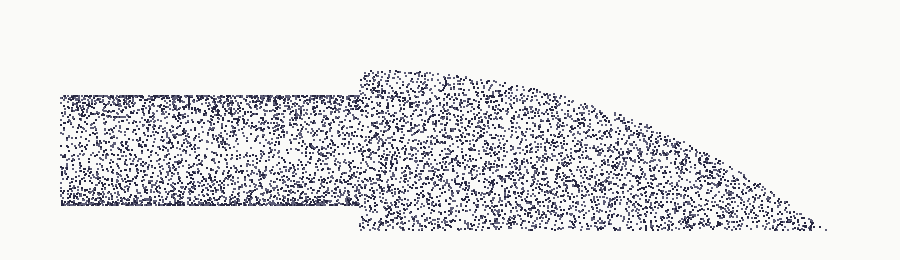
\includegraphics[width=0.75\linewidth]{figures/knife_scan_top.png}
\caption{Reference 3D scan of the knife (top view of the point cloud).}
\label{fig:knife}
\end{figure}

\begin{table}[htbp]
\centering\small
\begin{tabular}{@{}p{0.46\linewidth}cccc@{}}
\toprule
Query scan compared with the reference scan & RMS (mm) & P95 (mm) & Max (mm) & L2 verdict\\
\midrule
Same knife, re-scanned at FSL (new pose, new sampling, 0.15 mm noise) & 0.568 & 0.965 & 2.386 & MATCH\\
Same knife after an 8 x 5 mm nick appeared in the edge & 0.579 & 0.975 & 4.444 & \textbf{NO MATCH}\\
Same knife with 6 mm of the tip broken off & 0.570 & 0.964 & 5.024 & \textbf{NO MATCH}\\
Look-alike knife, blade 6 mm longer & 0.581 & 0.982 & 4.365 & \textbf{NO MATCH}\\
\bottomrule
\end{tabular}

\caption{3D-scan re-identification (rule: RMS $\le$ \KnifeRuleRms{} mm and maximum $\le$ \KnifeRuleMax{} mm).}
\label{tab:knife}
\end{table}

The RMS barely changes across all four cases, because it is dominated by sampling density, so a small local defect hardly moves it. The \emph{maximum} symmetric deviation is what reveals the 8$\times$5~mm nick, the broken tip and the 6~mm longer look-alike. Two lessons follow. The metric must be symmetric and must include a local term. And thresholds must be calibrated against the scanner's own repeatability: here the honest re-scan reaches a maximum of about 2.4~mm purely from sampling.

\subsection{Forensic image: acquisition verification and damage localisation}
\begin{table}[htbp]
\centering\small
\begin{tabular}{@{}ll@{}}
\toprule
Quantity & Value\\
\midrule
Source media size & 8{,}388{,}608 bytes (8 MiB)\\
SHA-256 of bit stream read during acquisition & \texttt{1b3166fa\allowbreak{}49149b5c\allowbreak{}3a2370e9\allowbreak{}d4242e60\ldots}\\
SHA-256 recomputed from finished image & \texttt{1b3166fa\allowbreak{}49149b5c\allowbreak{}3a2370e9\allowbreak{}d4242e60\ldots}\\
Acquisition verified (stream = image) & yes\\
SHA-256 of working copy with 1 bit flipped at byte 5{,}000{,}000 & \texttt{84b6d634\allowbreak{}e07837f5\allowbreak{}1604d601\allowbreak{}496e7489\ldots}\\
Chunk Merkle root (1 MiB chunks), good image & \texttt{e34fb65d\allowbreak{}b1bfba88\allowbreak{}0d50220a\allowbreak{}a447df5e\ldots}\\
Chunk Merkle root, corrupted copy & \texttt{bde2bf07\allowbreak{}c5c6c89d\allowbreak{}e6b98a40\allowbreak{}b8898912\ldots}\\
Chunks that differ (0-based) & 4 (bytes 4{,}194{,}304--5{,}242{,}879)\\
\bottomrule
\end{tabular}

\caption{Acquisition of an 8 MiB medium; a single bit flipped later in a working copy.}
\label{tab:disk}
\end{table}

The acquisition is verified when the hash of the stream read from the source equals the hash of the finished image. A single flipped bit in a later working copy changes the whole-file hash completely. The chunk Merkle tree localises the damage to one 1~MiB chunk, so the rest of the copy can still be shown to be intact.

\section{Limitations, risks and open questions}
\label{sec:limits}

\subsection{What the system cannot do}
\begin{enumerate}
  \item \textbf{Garbage in, garbage out at collection.} If a staged scene is photographed, a planted item is seized or a false description is written, the ledger preserves the falsehood faithfully. The mitigations are procedural (independent witnesses, continuous A/V recording under BNSS s.105, device-generated hashes, prompt anchoring), and the blockchain contributes nothing until the first hash is committed. This is also the observation of the reviewed literature on physical evidence~\cite{batista2023,patil2024}.
  \item \textbf{L2 is probabilistic.} The prototype now runs pHash and 3D comparisons itself (\cref{sec:impl}), but perceptual and geometric fingerprints have false-match and false-non-match rates that depend on the device, the operator, the object and the threshold. The thresholds in this document ($d_H \le 10$; RMS $\le$ \KnifeRuleRms{} mm, maximum $\le$ \KnifeRuleMax{} mm) were set on synthetic data and are illustrative only. Calibration on real captures, with measured error rates per evidence type, is required before any L2 result is reported as more than an examiner's aid.
  \item \textbf{Fine alterations of physical documents} (a changed digit, added strokes) are below the resolution of page-level fingerprints and remain a matter for questioned-document examination.
  \item \textbf{Items that legitimately change} (decay, swabbing, test-firing) require a new reference after each change; otherwise L2 comparisons against the original capture will fail for innocent reasons.
  \item \textbf{Collusion of a quorum.} BFT with four nodes tolerates one faulty agency, not two. Governance, meaning who operates which node and under what oversight, is as important as the protocol.
  \item \textbf{Key compromise.} A stolen officer certificate can sign false events. This requires certificate revocation, hardware-backed keys on capture devices, and a policy for retrospectively flagging events signed with a compromised key.
  \item \textbf{Prototype shortcuts.} Local passwords and in-memory sessions (D-043); one gateway holding every agency's storage master key (D-045); certificate authorities without TLS on localhost (D-035); hashing at upload rather than on the capture device (R1 partial).
  \item \textbf{Availability of the off-chain store.} The ledger proves integrity; it does not keep files alive. The master-negative store needs its own backup and replication policy (the SOP requires an off-site backup~\cite{sopbnss}).
\end{enumerate}

\subsection{Privacy}
Only fingerprints are on-chain. Artefact leaves are salted, so on-chain data cannot be used to test whether a known file belongs to a case. Personal data stays in the manifest, which is access-controlled and deletable off-chain. Fabric private data collections could restrict even manifest hashes to the agencies involved in a case. Whether this is necessary is an open question (O4 below).

\subsection{Algorithm agility}
Each artefact carries two digests from unrelated families. If one is weakened, records remain protected by the other, and a migration can add a new digest by registering a \code{DERIVE}d manifest that references the old one, without rewriting history.

\subsection{Open questions for discussion}
\begin{enumerate}[label=\textbf{O\arabic*}]
  \item \textbf{Scope of physical evidence for the prototype.} Which classes must be fully implemented first? Recommendation: scene photographs, A/V recordings, physical documents and physical items.
  \item \textbf{3D capture in practice.} Is a structured-light scanner realistic at the scene or the police station, or should photogrammetry from a phone, which is cheaper but less accurate, be the baseline?
  \item \textbf{Calibration data.} Can real (or realistic staged) captures be obtained to calibrate L2 thresholds and measure error rates?
  \item \textbf{Confidentiality between agencies.} Should all agencies see all ledger records, or should private data collections restrict records per case?
  \item \textbf{Integration with e-Sakshya.} Is an integration that consumes e-Sakshya's capture hashes a realistic target, or should the prototype provide its own capture app?
  \item \textbf{Legal review.} The points marked \emph{to verify} in \cref{sec:legal} need confirmation by a legal expert.
\end{enumerate}


\printbibliography[heading=bibintoc]

\appendix
\renewcommand{\thesection}{\Alph{section}}
\section{Input specification}
\label{app:spec}

This appendix is generated from \code{outputs/\allowbreak spec/\allowbreak evidence-manifest.schema.json} and \code{custody-event.schema.json} by \code{tools/schema\_to\_tex.py}, so it always matches the machine-readable specification. \enquote{Req.} marks fields the schema requires; a manifest missing any of them is rejected. General rules:
\begin{itemize}[nosep]
  \item timestamps are RFC~3339 with an explicit offset (e.g.\ \code{2026-11-19T10:42:05+05:30});
  \item decimals are strings, and floating-point numbers are forbidden so that canonicalisation is exact;
  \item persons who sign on the ledger carry their certificate subject (\code{pki\_subject});
  \item credentials (passcodes) are never recorded.
\end{itemize}

{\small
% Generated by outputs/tools/schema_to_tex.py from outputs/spec/*.schema.json -- do not edit by hand.
\subsection{Common blocks (all evidence classes)}
\subsubsection*{Manifest (top level)}
\begin{longtable}{@{}p{0.24\linewidth}p{0.07\linewidth}p{0.27\linewidth}p{0.36\linewidth}@{}}
\toprule Field & Req. & Type / allowed values & Meaning\\ \midrule\endhead
\texttt{spec\_version} & \textbf{yes} & = 1.0 & \\
\texttt{evidence\_id} & \textbf{yes} & string & Globally unique item ID: \textless{}STATE\textgreater{}-\textless{}DISTRICT\textgreater{}-\textless{}UNIT\textgreater{}-\textless{}YEAR\textgreater{}-\textless{}CASE SEQ\textgreater{}-E\textless{}ITEM SEQ\textgreater{}.\\
\texttt{parent\_evidence\_id} & no & string/null & Set when this item was derived from another item (aliquot, forensic image, extraction, enhanced copy).\\
\texttt{evidence\_class} & \textbf{yes} & enum (12 values) & \\
\texttt{title} & \textbf{yes} & string & \\
\texttt{description} & no & string & \\
\texttt{case} & \textbf{yes} & case & \\
\texttt{collection} & \textbf{yes} & collection & \\
\texttt{packaging} & \textbf{yes} & packaging & \\
\texttt{class\_attributes} & \textbf{yes} & object & \\
\texttt{artefacts} & \textbf{yes} & list of artefact & \\
\texttt{identity\_fingerprints} & no & list of identity\_fingerprint & Layer-2 (tolerant) fingerprints used to re-identify the physical item or content later. Never used as integrity proof.\\
\texttt{integrity} & \textbf{yes} & integrity & \\
\bottomrule
\end{longtable}

\subsubsection*{case}
\begin{longtable}{@{}p{0.24\linewidth}p{0.07\linewidth}p{0.27\linewidth}p{0.36\linewidth}@{}}
\toprule Field & Req. & Type / allowed values & Meaning\\ \midrule\endhead
\texttt{fir\_number} & \textbf{yes} & string & \\
\texttt{police\_station} & \textbf{yes} & string & \\
\texttt{district} & \textbf{yes} & string & \\
\texttt{state} & \textbf{yes} & string & \\
\texttt{sections\_invoked} & no & list of string & \\
\texttt{court} & no & string & \\
\texttt{cctns\_case\_id} & no & string & \\
\bottomrule
\end{longtable}

\subsubsection*{collection}
\begin{longtable}{@{}p{0.24\linewidth}p{0.07\linewidth}p{0.27\linewidth}p{0.36\linewidth}@{}}
\toprule Field & Req. & Type / allowed values & Meaning\\ \midrule\endhead
\texttt{collected\_at} & \textbf{yes} & timestamp & RFC 3339 with explicit offset, e.g. 2026-11-19T10:42:05+05:30.\\
\texttt{location} & \textbf{yes} & location & \\
\texttt{collected\_by} & \textbf{yes} & person & \\
\texttt{witnesses} & no & list of person & \\
\texttt{legal\_basis} & \textbf{yes} & string & e.g. 'BNSS s.105 search and seizure', 'BNSS s.176(3) forensic scene visit', 'BNSS s.94 production'.\\
\texttt{seizure\_memo\_ref} & no & string & evidence\_id of the PROCEDURAL\_DOCUMENT holding the seizure memo / panchnama.\\
\texttt{av\_recording\_ref} & no & string & evidence\_id of the AV\_RECORDING of the search/seizure (BNSS s.105).\\
\texttt{condition\_on\_collection} & no & string & \\
\bottomrule
\end{longtable}

\subsubsection*{packaging}
\begin{longtable}{@{}p{0.24\linewidth}p{0.07\linewidth}p{0.27\linewidth}p{0.36\linewidth}@{}}
\toprule Field & Req. & Type / allowed values & Meaning\\ \midrule\endhead
\texttt{container} & \textbf{yes} & string & e.g. 'tamper-evident bag', 'Faraday bag', 'sealed envelope', 'cold-chain box', 'none (born-digital)'\\
\texttt{seal\_ids} & no & list of string & \\
\texttt{label\_id} & no & string & Printed label / QR / RFID identifier affixed to the container.\\
\texttt{sealed\_by} & no & person & \\
\texttt{sealed\_at} & no & timestamp & RFC 3339 with explicit offset, e.g. 2026-11-19T10:42:05+05:30.\\
\bottomrule
\end{longtable}

\subsubsection*{artefacts[] (one per captured file)}
\begin{longtable}{@{}p{0.24\linewidth}p{0.07\linewidth}p{0.27\linewidth}p{0.36\linewidth}@{}}
\toprule Field & Req. & Type / allowed values & Meaning\\ \midrule\endhead
\texttt{artefact\_id} & \textbf{yes} & string & \\
\texttt{sequence} & no & integer & Order of the artefact within the item (page number, frame number, segment number).\\
\texttt{role} & \textbf{yes} & enum (27 values) & \\
\texttt{media\_type} & \textbf{yes} & string & IANA media type, e.g. image/jpeg, model/ply, application/pdf.\\
\texttt{file\_name} & no & string & \\
\texttt{size\_bytes} & \textbf{yes} & integer & \\
\texttt{sha256} & \textbf{yes} & hex (64) & \\
\texttt{sha3\_256} & \textbf{yes} & hex (64) & \\
\texttt{hashed\_at} & no & timestamp & RFC 3339 with explicit offset, e.g. 2026-11-19T10:42:05+05:30.\\
\texttt{hashed\_on} & no & string & Where the first hash was computed: 'capture device', 'police station designated desktop', 'FSL workstation'.\\
\texttt{captured\_at} & \textbf{yes} & timestamp & RFC 3339 with explicit offset, e.g. 2026-11-19T10:42:05+05:30.\\
\texttt{capture\_device} & \textbf{yes} & device & Mirrors the device fields of the BSA s.63(4)(c) Schedule certificate.\\
\texttt{capture\_parameters} & no & object & Class-specific capture settings (dpi, resolution, codec, scanner accuracy, ...).\\
\texttt{parent\_artefact\_id} & no & string/null & Set for a derived artefact (enhanced copy, transcode); the original must remain in the manifest.\\
\texttt{chunking} & no & object\{chunk\_size\_bytes, chunk\_merkle\_root\} & Optional chunk-level hashes for large files (video, images) so damage can be localised.\\
\texttt{leaf\_salt} & no & string & 32-byte random salt for this artefact's Merkle leaf (kept off-chain).\\
\bottomrule
\end{longtable}

\subsubsection*{capture\_device (mirrors the BSA s.63(4)(c) Schedule)}
\begin{longtable}{@{}p{0.24\linewidth}p{0.07\linewidth}p{0.27\linewidth}p{0.36\linewidth}@{}}
\toprule Field & Req. & Type / allowed values & Meaning\\ \midrule\endhead
\texttt{device\_type} & \textbf{yes} & one of: Computer/Storage Media, DVR, Mobile, Flash Drive, CD/DVD, Server, Cloud, Camera, 3D Scanner, Flatbed Scanner, Other & \\
\texttt{make\_model} & \textbf{yes} & string & \\
\texttt{colour} & no & string & \\
\texttt{serial\_number} & no & string & \\
\texttt{imei\_uin\_uid\_mac\_cloud\_id} & no & string & \\
\texttt{software} & no & string & Capture app / firmware and version, e.g. 'e-Sakshya 2.x'.\\
\texttt{clock\_check} & no & object\{reference, offset\_seconds\} & \\
\bottomrule
\end{longtable}

\subsubsection*{person}
\begin{longtable}{@{}p{0.24\linewidth}p{0.07\linewidth}p{0.27\linewidth}p{0.36\linewidth}@{}}
\toprule Field & Req. & Type / allowed values & Meaning\\ \midrule\endhead
\texttt{name} & \textbf{yes} & string & \\
\texttt{role} & \textbf{yes} & string & e.g. Investigating Officer, First Responder, FSL Examiner, Independent Witness\\
\texttt{designation} & no & string & \\
\texttt{badge\_or\_employee\_id} & no & string & \\
\texttt{organisation} & no & string & \\
\texttt{pki\_subject} & no & string & X.509 subject DN of the signing certificate (Fabric identity) when the person signs on the ledger.\\
\texttt{address} & no & string & Required for independent witnesses (BNSS search witnesses).\\
\bottomrule
\end{longtable}

\subsubsection*{identity\_fingerprints[]}
\begin{longtable}{@{}p{0.24\linewidth}p{0.07\linewidth}p{0.27\linewidth}p{0.36\linewidth}@{}}
\toprule Field & Req. & Type / allowed values & Meaning\\ \midrule\endhead
\texttt{method} & \textbf{yes} & one of: phash-dct-64, dhash-64, mesh-icp-rms, seal-id-exact, label-id-exact, serial-exact, keypoint-set, measurement-tolerance & \\
\texttt{method\_version} & \textbf{yes} & string & \\
\texttt{source\_artefact\_ids} & \textbf{yes} & list of string & \\
\texttt{value} & \textbf{yes} & string & Fingerprint value (hex for hashes; for mesh-icp-rms the SHA-256 of the reference mesh).\\
\texttt{match\_rule} & \textbf{yes} & string & Machine-readable acceptance rule, e.g. 'hamming\textless{}=10', 'rms\_mm\textless{}=0.50', 'exact'.\\
\bottomrule
\end{longtable}

\subsection{Class-specific attributes (\texttt{class\_attributes})}
\subsubsection*{SCENE\_PHOTOGRAPH}
\begin{longtable}{@{}p{0.24\linewidth}p{0.07\linewidth}p{0.27\linewidth}p{0.36\linewidth}@{}}
\toprule Field & Req. & Type / allowed values & Meaning\\ \midrule\endhead
\texttt{photo\_series\_id} & \textbf{yes} & string & \\
\texttt{frame\_number} & \textbf{yes} & integer & \\
\texttt{view} & \textbf{yes} & one of: overall, mid-range, close-up, aerial, entry-exit & \\
\texttt{scale\_present} & \textbf{yes} & boolean & \\
\texttt{colour\_reference\_present} & no & boolean & \\
\texttt{subject} & \textbf{yes} & string & \\
\texttt{original\_format} & no & one of: JPEG, HEIC, RAW-DNG, RAW-VENDOR, PNG, TIFF & \\
\texttt{flash} & no & boolean & \\
\bottomrule
\end{longtable}

\subsubsection*{AV\_RECORDING}
\begin{longtable}{@{}p{0.24\linewidth}p{0.07\linewidth}p{0.27\linewidth}p{0.36\linewidth}@{}}
\toprule Field & Req. & Type / allowed values & Meaning\\ \midrule\endhead
\texttt{purpose} & \textbf{yes} & one of: search-seizure, scene-of-crime, witness-statement, victim-statement, identification-parade, property-disposal, other & \\
\texttt{legal\_provision} & \textbf{yes} & string & e.g. 'BNSS s.105', 'BNSS s.185(2)', 'BNSS s.176(3)', 'BNSS s.180(3)'\\
\texttt{started\_at} & \textbf{yes} & timestamp & RFC 3339 with explicit offset, e.g. 2026-11-19T10:42:05+05:30.\\
\texttt{ended\_at} & \textbf{yes} & timestamp & RFC 3339 with explicit offset, e.g. 2026-11-19T10:42:05+05:30.\\
\texttt{media\_blank\_confirmed} & \textbf{yes} & boolean & \\
\texttt{segment\_number} & \textbf{yes} & integer & \\
\texttt{segment\_count} & \textbf{yes} & integer & \\
\texttt{continuity\_device\_ref} & no & string & evidence\_id of the second recorder that captured a memory-card change, if any.\\
\texttt{codec} & no & string & \\
\texttt{forwarded\_to\_magistrate\_at} & no & timestamp & RFC 3339 with explicit offset, e.g. 2026-11-19T10:42:05+05:30.\\
\bottomrule
\end{longtable}

\subsubsection*{CCTV\_EXPORT}
\begin{longtable}{@{}p{0.24\linewidth}p{0.07\linewidth}p{0.27\linewidth}p{0.36\linewidth}@{}}
\toprule Field & Req. & Type / allowed values & Meaning\\ \midrule\endhead
\texttt{system\_make\_model} & \textbf{yes} & string & \\
\texttt{system\_serial} & no & string & \\
\texttt{owner\_or\_operator} & no & person & \\
\texttt{camera\_ids} & \textbf{yes} & list of string & \\
\texttt{footage\_start} & \textbf{yes} & timestamp & RFC 3339 with explicit offset, e.g. 2026-11-19T10:42:05+05:30.\\
\texttt{footage\_end} & \textbf{yes} & timestamp & RFC 3339 with explicit offset, e.g. 2026-11-19T10:42:05+05:30.\\
\texttt{dvr\_clock\_offset\_seconds} & \textbf{yes} & integer & \\
\texttt{export\_method} & \textbf{yes} & string & \\
\texttt{native\_format} & no & string & \\
\texttt{native\_player\_included} & no & boolean & \\
\bottomrule
\end{longtable}

\subsubsection*{PHYSICAL\_DOCUMENT}
\begin{longtable}{@{}p{0.24\linewidth}p{0.07\linewidth}p{0.27\linewidth}p{0.36\linewidth}@{}}
\toprule Field & Req. & Type / allowed values & Meaning\\ \midrule\endhead
\texttt{document\_type} & \textbf{yes} & string & e.g. 'spiral notebook', 'ledger', 'letter', 'diary'\\
\texttt{page\_count} & \textbf{yes} & integer & Number of sides scanned (each side is one page\_scan artefact).\\
\texttt{leaf\_count} & no & integer & \\
\texttt{blank\_pages} & no & list of integer & \\
\texttt{dimensions\_mm} & \textbf{yes} & object\{width, height, thickness\} & \\
\texttt{binding} & \textbf{yes} & string & \\
\texttt{writing\_media} & no & list of string & \\
\texttt{distinguishing\_features} & \textbf{yes} & list of string & \\
\texttt{scan\_dpi} & \textbf{yes} & integer & \\
\texttt{scan\_colour\_mode} & \textbf{yes} & one of: RGB-24, RGB-48, GRAY-8, GRAY-16 & \\
\texttt{scan\_file\_format} & no & one of: PNG, TIFF & \\
\bottomrule
\end{longtable}

\subsubsection*{PHYSICAL\_ITEM}
\begin{longtable}{@{}p{0.24\linewidth}p{0.07\linewidth}p{0.27\linewidth}p{0.36\linewidth}@{}}
\toprule Field & Req. & Type / allowed values & Meaning\\ \midrule\endhead
\texttt{item\_category} & \textbf{yes} & string & e.g. 'edged weapon', 'firearm', 'garment', 'footwear', 'tool'\\
\texttt{dimensions\_mm} & \textbf{yes} & object\{length, width, height\} & \\
\texttt{mass} & no & quantity & \\
\texttt{material} & \textbf{yes} & string & \\
\texttt{colour} & no & string & \\
\texttt{serial\_or\_make\_marks} & no & string & \\
\texttt{unique\_marks} & \textbf{yes} & list of string & \\
\texttt{scan\_3d} & \textbf{yes} & object\{method, point\_spacing\_mm, stated\_accuracy\_mm, reason\_not\_performed\} & \\
\texttt{expected\_changes} & no & list of string & Known reasons the item may legitimately change (swabbing, decay, test firing).\\
\bottomrule
\end{longtable}

\subsubsection*{BIO\_TRACE\_SAMPLE}
\begin{longtable}{@{}p{0.24\linewidth}p{0.07\linewidth}p{0.27\linewidth}p{0.36\linewidth}@{}}
\toprule Field & Req. & Type / allowed values & Meaning\\ \midrule\endhead
\texttt{sample\_type} & \textbf{yes} & string & e.g. 'blood swab', 'hair', 'soil', 'fibre', 'viscera'\\
\texttt{collection\_method} & \textbf{yes} & string & \\
\texttt{container\_type} & \textbf{yes} & string & \\
\texttt{container\_barcode} & \textbf{yes} & string & \\
\texttt{quantity} & \textbf{yes} & quantity & \\
\texttt{storage\_condition} & \textbf{yes} & one of: ambient, refrigerated-2-8C, frozen--20C, frozen--80C, dry & \\
\texttt{temperature\_log\_ref} & no & string & \\
\texttt{biohazard} & no & boolean & \\
\texttt{consumed\_by\_testing} & no & boolean & \\
\bottomrule
\end{longtable}

\subsubsection*{DIGITAL\_DEVICE}
\begin{longtable}{@{}p{0.24\linewidth}p{0.07\linewidth}p{0.27\linewidth}p{0.36\linewidth}@{}}
\toprule Field & Req. & Type / allowed values & Meaning\\ \midrule\endhead
\texttt{device\_type} & \textbf{yes} & one of: Computer/Storage Media, DVR, Mobile, Flash Drive, CD/DVD, Server, Other & \\
\texttt{make\_model} & \textbf{yes} & string & \\
\texttt{colour} & no & string & \\
\texttt{serial\_number} & \textbf{yes} & string & \\
\texttt{imei\_uin\_uid\_mac} & no & list of string & \\
\texttt{sim\_iccids} & no & list of string & \\
\texttt{storage\_media} & no & list of string & \\
\texttt{power\_state\_at\_seizure} & \textbf{yes} & one of: on-unlocked, on-locked, off, unknown & \\
\texttt{isolation} & \textbf{yes} & one of: faraday-bag, airplane-mode, powered-off, none & \\
\texttt{lock\_status} & no & one of: no-lock, locked-credential-known, locked-credential-unknown & Never store the credential itself in the manifest.\\
\bottomrule
\end{longtable}

\subsubsection*{FORENSIC\_IMAGE}
\begin{longtable}{@{}p{0.24\linewidth}p{0.07\linewidth}p{0.27\linewidth}p{0.36\linewidth}@{}}
\toprule Field & Req. & Type / allowed values & Meaning\\ \midrule\endhead
\texttt{acquisition\_tool} & \textbf{yes} & string & Name and exact version.\\
\texttt{write\_blocker} & \textbf{yes} & string & Make, model and serial, or 'software (name/version)' or 'none (justify)'.\\
\texttt{image\_format} & \textbf{yes} & one of: RAW-DD, E01, EX01, AFF4, VENDOR & \\
\texttt{source\_media\_size\_bytes} & no & integer & \\
\texttt{source\_stream\_sha256} & \textbf{yes} & hex (64) & SHA-256 of the bit stream read from the source media during acquisition.\\
\texttt{verification\_sha256} & \textbf{yes} & hex (64) & SHA-256 recomputed from the finished image; must equal source\_stream\_sha256.\\
\texttt{tool\_reported\_hashes} & no & object & Hashes reported by the tool (e.g. E01 embedded MD5/SHA-1), kept for cross-reference only.\\
\texttt{bad\_sectors} & no & integer & \\
\texttt{acquisition\_started\_at} & \textbf{yes} & timestamp & RFC 3339 with explicit offset, e.g. 2026-11-19T10:42:05+05:30.\\
\texttt{acquisition\_ended\_at} & \textbf{yes} & timestamp & RFC 3339 with explicit offset, e.g. 2026-11-19T10:42:05+05:30.\\
\texttt{examiner} & \textbf{yes} & person & \\
\bottomrule
\end{longtable}

\subsubsection*{MOBILE\_EXTRACTION}
\begin{longtable}{@{}p{0.24\linewidth}p{0.07\linewidth}p{0.27\linewidth}p{0.36\linewidth}@{}}
\toprule Field & Req. & Type / allowed values & Meaning\\ \midrule\endhead
\texttt{tool} & \textbf{yes} & string & Name and exact version.\\
\texttt{extraction\_type} & \textbf{yes} & one of: logical, file-system, full-file-system, physical, cloud-token & \\
\texttt{device\_state} & no & string & \\
\texttt{started\_at} & \textbf{yes} & timestamp & RFC 3339 with explicit offset, e.g. 2026-11-19T10:42:05+05:30.\\
\texttt{ended\_at} & \textbf{yes} & timestamp & RFC 3339 with explicit offset, e.g. 2026-11-19T10:42:05+05:30.\\
\texttt{tool\_reported\_hashes} & no & object & \\
\texttt{examiner} & \textbf{yes} & person & \\
\bottomrule
\end{longtable}

\subsubsection*{CLOUD\_DATA}
\begin{longtable}{@{}p{0.24\linewidth}p{0.07\linewidth}p{0.27\linewidth}p{0.36\linewidth}@{}}
\toprule Field & Req. & Type / allowed values & Meaning\\ \midrule\endhead
\texttt{provider} & \textbf{yes} & string & \\
\texttt{account\_identifiers} & \textbf{yes} & list of string & \\
\texttt{legal\_process\_ref} & \textbf{yes} & string & Notice / order reference under which the data was produced.\\
\texttt{date\_range\_requested} & no & object\{from, to\} & \\
\texttt{received\_at} & \textbf{yes} & timestamp & RFC 3339 with explicit offset, e.g. 2026-11-19T10:42:05+05:30.\\
\texttt{delivery\_method} & \textbf{yes} & string & \\
\texttt{provider\_supplied\_hash} & no & string & \\
\texttt{provider\_signature\_present} & no & boolean & \\
\texttt{capture\_format} & no & one of: provider-native, WARC, PDF-print, JSON, CSV, other & \\
\bottomrule
\end{longtable}

\subsubsection*{IOT\_LOG}
\begin{longtable}{@{}p{0.24\linewidth}p{0.07\linewidth}p{0.27\linewidth}p{0.36\linewidth}@{}}
\toprule Field & Req. & Type / allowed values & Meaning\\ \midrule\endhead
\texttt{source\_system} & \textbf{yes} & string & \\
\texttt{device\_ids} & \textbf{yes} & list of string & \\
\texttt{log\_start} & \textbf{yes} & timestamp & RFC 3339 with explicit offset, e.g. 2026-11-19T10:42:05+05:30.\\
\texttt{log\_end} & \textbf{yes} & timestamp & RFC 3339 with explicit offset, e.g. 2026-11-19T10:42:05+05:30.\\
\texttt{time\_sync} & \textbf{yes} & string & e.g. 'NTP pool, $\pm$50 ms', 'unsynchronised RTC (offset measured: +312 s)'\\
\texttt{at\_source\_integrity} & \textbf{yes} & one of: hash-chained, signed, append-only-store, none & \\
\texttt{export\_method} & no & string & \\
\texttt{log\_format} & no & string & \\
\bottomrule
\end{longtable}

\subsubsection*{PROCEDURAL\_DOCUMENT}
\begin{longtable}{@{}p{0.24\linewidth}p{0.07\linewidth}p{0.27\linewidth}p{0.36\linewidth}@{}}
\toprule Field & Req. & Type / allowed values & Meaning\\ \midrule\endhead
\texttt{document\_type} & \textbf{yes} & enum (11 values) & \\
\texttt{document\_number} & \textbf{yes} & string & \\
\texttt{born\_digital} & \textbf{yes} & boolean & \\
\texttt{signatories} & \textbf{yes} & list of person & \\
\texttt{digital\_signature} & no & string & e.g. 'IT Act 2000 s.3A electronic signature (eSign)', 'none'\\
\texttt{refers\_to\_evidence\_ids} & no & list of string & \\
\bottomrule
\end{longtable}

\subsection{Custody event}
\subsubsection*{custody event (submitted to the chaincode)}
\begin{longtable}{@{}p{0.24\linewidth}p{0.07\linewidth}p{0.27\linewidth}p{0.36\linewidth}@{}}
\toprule Field & Req. & Type / allowed values & Meaning\\ \midrule\endhead
\texttt{spec\_version} & \textbf{yes} & = 1.0 & \\
\texttt{evidence\_id} & \textbf{yes} & string & \\
\texttt{event\_type} & \textbf{yes} & enum (17 values) & \\
\texttt{reason} & \textbf{yes} & string & Why the event happened (the 'Why' of 5W1H), e.g. court order number, FSL request number.\\
\texttt{location} & no & string & \\
\texttt{manifest\_sha256} & no & string & REGISTER, DERIVE: SHA-256 of the RFC 8785 canonical manifest.\\
\texttt{merkle\_root} & no & string & REGISTER, DERIVE: salted RFC 6962 Merkle root over the manifest's artefacts.\\
\texttt{to\_org\_msp} & no & string & TRANSFER\_INITIATE: receiving organisation, e.g. FSLMSP.\\
\texttt{to\_custodian\_subject} & no & string & TRANSFER\_INITIATE: X.509 subject of the intended receiving custodian.\\
\texttt{transfer\_ref} & no & string & TRANSFER\_ACCEPT/REJECT: tx id of the matching TRANSFER\_INITIATE.\\
\texttt{seal\_ids\_observed} & no & list of string & SEAL, TRANSFER\_ACCEPT, RESEAL, VERIFY\_IDENTITY: seal numbers read on the package.\\
\texttt{seal\_intact} & no & boolean & TRANSFER\_ACCEPT, VERIFY\_IDENTITY: seal condition on receipt.\\
\texttt{child\_evidence\_id} & no & string & DERIVE: the new item (forensic image, aliquot, extraction, enhanced copy).\\
\texttt{verification} & no & object\{method, method\_version, result, score, threshold, query\_artefact\_sha256\} & VERIFY\_INTEGRITY / VERIFY\_IDENTITY result.\\
\texttt{attachments\_sha256} & no & list of string & Hashes of documents created by this event (receipt photo, FSL report, court order).\\
\texttt{corrects\_event\_tx} & no & string & CORRECTION: tx id of the event being corrected.\\
\bottomrule
\end{longtable}


}

\subsection{Example manifest}
The complete manifest of the scene photograph used in \cref{sec:worked} (\code{spec/\allowbreak examples/\allowbreak scene-photo.manifest.json}):
\lstinputlisting[style=json]{../spec/examples/scene-photo.manifest.json}

\section{Reproducing the results}
\label{app:repro}

\begin{lstlisting}[style=json,language=bash]
cd outputs
python3 tools/make_worked_examples.py        # artefacts, manifests, tables, figures
python3 tools/schema_to_tex.py               # Appendix A from the JSON Schemas
cd report && latexmk -pdf main.tex            # this document

# Independent checks with the reference tool
python3 tools/evidence_hash.py validate spec/examples/notebook.manifest.json
python3 tools/evidence_hash.py verify   spec/examples/notebook.manifest.json --base worked-example/files
python3 tools/evidence_hash.py prove    spec/examples/notebook.manifest.json A006
python3 tools/evidence_hash.py compare-images worked-example/files/photo/IMG_0001.jpg \
                                              worked-example/files/photo/IMG_0001_knife_removed.jpg
python3 tools/evidence_hash.py compare-mesh worked-example/files/knife/reference_scan.ply \
                                            worked-example/files/knife/rescan_notched.ply
sha256sum worked-example/files/photo/IMG_0001.jpg   # any standard tool gives the same L1 hash
\end{lstlisting}

Requirements: Python 3 with \code{numpy}, \code{Pillow}, \code{jsonschema} (and optionally \code{scipy} for faster 3D comparison); a \TeX{} distribution with \code{biber}. The generated evidence files are deterministic for a given library version but are not stored in the repository; re-running the generator recreates them.


\end{document}
